\documentclass[12pt,a4paper,titlepage]{scrartcl}

\usepackage{comment}
\usepackage[main=ngerman,english]{babel}
\usepackage[utf8]{inputenc}
\usepackage[T1]{fontenc}
\usepackage{lmodern}
\usepackage{geometry}
\geometry{left=2.5cm,right=2.5cm,top=2.5cm,bottom=3cm,head=29pt,foot=25pt}
\setlength{\footheight}{25pt}
\usepackage{microtype}
\usepackage{amsmath,amssymb,mathtools}
\numberwithin{equation}{section}
\numberwithin{table}{section}
\numberwithin{figure}{section}
\usepackage{siunitx}
\sisetup{locale=US, separate-uncertainty=true, per-mode=fraction}
\usepackage{booktabs}
\usepackage{multirow}
\usepackage{graphicx}
\usepackage{float}
\usepackage{caption}
\usepackage{subcaption}
\usepackage[automark]{scrlayer-scrpage}
\usepackage[most]{tcolorbox}
\usepackage{hyperref}
\usepackage{pdfpages}
\usepackage{csvsimple-l3}
\usepackage{longtable}


% Basic figure setup, for now with no caption control since it's done
% automatically by Pandoc (which extracts ![](path) syntax from Markdown).
\usepackage{graphicx}
% Keep aspect ratio if custom image width or height is specified
\setkeys{Gin}{keepaspectratio}
% Maintain compatibility with old templates. Remove in nbconvert 6.0
\let\Oldincludegraphics\includegraphics
\usepackage{caption}

\usepackage{float}

\floatplacement{figure}{H} % forces figures to be placed at the correct location
\usepackage{xcolor} % Allow colors to be defined
\usepackage{enumerate} % Needed for markdown enumerations to work
\usepackage{geometry} % Used to adjust the document margins
\usepackage{amsmath} % Equations
\usepackage{amssymb} % Equations
\usepackage{textcomp} % defines textquotesingle
% Hack from http://tex.stackexchange.com/a/47451/13684:
\AtBeginDocument{%
    \def\PYZsq{\textquotesingle}% Upright quotes in Pygmentized code
}
\usepackage{upquote} % Upright quotes for verbatim code
\usepackage{eurosym} % defines \euro

\usepackage{iftex}
\ifPDFTeX
    \usepackage[T1]{fontenc}
    \IfFileExists{alphabeta.sty}{
            \usepackage{alphabeta}
        }{
            \usepackage[mathletters]{ucs}
            \usepackage[utf8x]{inputenc}
        }
\else
    \usepackage{fontspec}
    \usepackage{unicode-math}
\fi

\usepackage{fancyvrb} % verbatim replacement that allows latex
\usepackage{grffile} % extends the file name processing of package graphics
                        % to support a larger range
\makeatletter % fix for old versions of grffile with XeLaTeX
\@ifpackagelater{grffile}{2019/11/01}
{
    % Do nothing on new versions
}
{
    \def\Gread@@xetex#1{%
    \IfFileExists{"\Gin@base".bb}%
    {\Gread@eps{\Gin@base.bb}}%
    {\Gread@@xetex@aux#1}%
    }
}
\makeatother
\usepackage[Export]{adjustbox} % Used to constrain images to a maximum size
\adjustboxset{max size={0.9\linewidth}{0.9\paperheight}}

% The hyperref package gives us a pdf with properly built
% internal navigation ('pdf bookmarks' for the table of contents,
% internal cross-reference links, web links for URLs, etc.)
\usepackage{hyperref}
% The default LaTeX title has an obnoxious amount of whitespace. By default,
% titling removes some of it. It also provides customization options.
\usepackage{titling}
\usepackage{longtable} % longtable support required by pandoc >1.10
\usepackage{booktabs}  % table support for pandoc > 1.12.2
\usepackage{array}     % table support for pandoc >= 2.11.3
\usepackage{calc}      % table minipage width calculation for pandoc >= 2.11.1
\usepackage[inline]{enumitem} % IRkernel/repr support (it uses the enumerate* environment)
\usepackage[normalem]{ulem} % ulem is needed to support strikethroughs (\sout)
                            % normalem makes italics be italics, not underlines
\usepackage{soul}      % strikethrough (\st) support for pandoc >= 3.0.0
\usepackage{mathrsfs}



% Colors for the hyperref package
\definecolor{urlcolor}{rgb}{0,.145,.698}
\definecolor{linkcolor}{rgb}{.71,0.21,0.01}
\definecolor{citecolor}{rgb}{.12,.54,.11}

% ANSI colors
\definecolor{ansi-black}{HTML}{3E424D}
\definecolor{ansi-black-intense}{HTML}{282C36}
\definecolor{ansi-red}{HTML}{E75C58}
\definecolor{ansi-red-intense}{HTML}{B22B31}
\definecolor{ansi-green}{HTML}{00A250}
\definecolor{ansi-green-intense}{HTML}{007427}
\definecolor{ansi-yellow}{HTML}{DDB62B}
\definecolor{ansi-yellow-intense}{HTML}{B27D12}
\definecolor{ansi-blue}{HTML}{208FFB}
\definecolor{ansi-blue-intense}{HTML}{0065CA}
\definecolor{ansi-magenta}{HTML}{D160C4}
\definecolor{ansi-magenta-intense}{HTML}{A03196}
\definecolor{ansi-cyan}{HTML}{60C6C8}
\definecolor{ansi-cyan-intense}{HTML}{258F8F}
\definecolor{ansi-white}{HTML}{C5C1B4}
\definecolor{ansi-white-intense}{HTML}{A1A6B2}
\definecolor{ansi-default-inverse-fg}{HTML}{FFFFFF}
\definecolor{ansi-default-inverse-bg}{HTML}{000000}

% common color for the border for error outputs.
\definecolor{outerrorbackground}{HTML}{FFDFDF}

% commands and environments needed by pandoc snippets
% extracted from the output of `pandoc -s`
\providecommand{\tightlist}{%
    \setlength{\itemsep}{0pt}\setlength{\parskip}{0pt}}
\DefineVerbatimEnvironment{Highlighting}{Verbatim}{commandchars=\\\{\}}
% Add ',fontsize=\small' for more characters per line
\newenvironment{Shaded}{}{}
\newcommand{\KeywordTok}[1]{\textcolor[rgb]{0.00,0.44,0.13}{\textbf{{#1}}}}
\newcommand{\DataTypeTok}[1]{\textcolor[rgb]{0.56,0.13,0.00}{{#1}}}
\newcommand{\DecValTok}[1]{\textcolor[rgb]{0.25,0.63,0.44}{{#1}}}
\newcommand{\BaseNTok}[1]{\textcolor[rgb]{0.25,0.63,0.44}{{#1}}}
\newcommand{\FloatTok}[1]{\textcolor[rgb]{0.25,0.63,0.44}{{#1}}}
\newcommand{\CharTok}[1]{\textcolor[rgb]{0.25,0.44,0.63}{{#1}}}
\newcommand{\StringTok}[1]{\textcolor[rgb]{0.25,0.44,0.63}{{#1}}}
\newcommand{\CommentTok}[1]{\textcolor[rgb]{0.38,0.63,0.69}{\textit{{#1}}}}
\newcommand{\OtherTok}[1]{\textcolor[rgb]{0.00,0.44,0.13}{{#1}}}
\newcommand{\AlertTok}[1]{\textcolor[rgb]{1.00,0.00,0.00}{\textbf{{#1}}}}
\newcommand{\FunctionTok}[1]{\textcolor[rgb]{0.02,0.16,0.49}{{#1}}}
\newcommand{\RegionMarkerTok}[1]{{#1}}
\newcommand{\ErrorTok}[1]{\textcolor[rgb]{1.00,0.00,0.00}{\textbf{{#1}}}}
\newcommand{\NormalTok}[1]{{#1}}

% Additional commands for more recent versions of Pandoc
\newcommand{\ConstantTok}[1]{\textcolor[rgb]{0.53,0.00,0.00}{{#1}}}
\newcommand{\SpecialCharTok}[1]{\textcolor[rgb]{0.25,0.44,0.63}{{#1}}}
\newcommand{\VerbatimStringTok}[1]{\textcolor[rgb]{0.25,0.44,0.63}{{#1}}}
\newcommand{\SpecialStringTok}[1]{\textcolor[rgb]{0.73,0.40,0.53}{{#1}}}
\newcommand{\ImportTok}[1]{{#1}}
\newcommand{\DocumentationTok}[1]{\textcolor[rgb]{0.73,0.13,0.13}{\textit{{#1}}}}
\newcommand{\AnnotationTok}[1]{\textcolor[rgb]{0.38,0.63,0.69}{\textbf{\textit{{#1}}}}}
\newcommand{\CommentVarTok}[1]{\textcolor[rgb]{0.38,0.63,0.69}{\textbf{\textit{{#1}}}}}
\newcommand{\VariableTok}[1]{\textcolor[rgb]{0.10,0.09,0.49}{{#1}}}
\newcommand{\ControlFlowTok}[1]{\textcolor[rgb]{0.00,0.44,0.13}{\textbf{{#1}}}}
\newcommand{\OperatorTok}[1]{\textcolor[rgb]{0.40,0.40,0.40}{{#1}}}
\newcommand{\BuiltInTok}[1]{{#1}}
\newcommand{\ExtensionTok}[1]{{#1}}
\newcommand{\PreprocessorTok}[1]{\textcolor[rgb]{0.74,0.48,0.00}{{#1}}}
\newcommand{\AttributeTok}[1]{\textcolor[rgb]{0.49,0.56,0.16}{{#1}}}
\newcommand{\InformationTok}[1]{\textcolor[rgb]{0.38,0.63,0.69}{\textbf{\textit{{#1}}}}}
\newcommand{\WarningTok}[1]{\textcolor[rgb]{0.38,0.63,0.69}{\textbf{\textit{{#1}}}}}
\makeatletter
\newsavebox\pandoc@box
\newcommand*\pandocbounded[1]{%
    \sbox\pandoc@box{#1}%
    % scaling factors for width and height
    \Gscale@div\@tempa\textheight{\dimexpr\ht\pandoc@box+\dp\pandoc@box\relax}%
    \Gscale@div\@tempb\linewidth{\wd\pandoc@box}%
    % select the smaller of both
    \ifdim\@tempb\p@<\@tempa\p@
    \let\@tempa\@tempb
    \fi
    % scaling accordingly (\@tempa < 1)
    \ifdim\@tempa\p@<\p@
    \scalebox{\@tempa}{\usebox\pandoc@box}%
    % scaling not needed, use as it is
    \else
    \usebox{\pandoc@box}%
    \fi
}
\makeatother

% Define a nice break command that doesn't care if a line doesn't already
% exist.
\def\br{\hspace*{\fill} \\* }
% Math Jax compatibility definitions
\def\gt{>}
\def\lt{<}
\let\Oldtex\TeX
\let\Oldlatex\LaTeX
\renewcommand{\TeX}{\textrm{\Oldtex}}
\renewcommand{\LaTeX}{\textrm{\Oldlatex}}
% Document parameters
% Document title
\title{U-I-Diagramm}
    

    
    
    
    
    
% Pygments definitions
\makeatletter
\def\PY@reset{\let\PY@it=\relax \let\PY@bf=\relax%
    \let\PY@ul=\relax \let\PY@tc=\relax%
    \let\PY@bc=\relax \let\PY@ff=\relax}
\def\PY@tok#1{\csname PY@tok@#1\endcsname}
\def\PY@toks#1+{\ifx\relax#1\empty\else%
    \PY@tok{#1}\expandafter\PY@toks\fi}
\def\PY@do#1{\PY@bc{\PY@tc{\PY@ul{%
    \PY@it{\PY@bf{\PY@ff{#1}}}}}}}
\def\PY#1#2{\PY@reset\PY@toks#1+\relax+\PY@do{#2}}

\@namedef{PY@tok@w}{\def\PY@tc##1{\textcolor[rgb]{0.73,0.73,0.73}{##1}}}
\@namedef{PY@tok@c}{\let\PY@it=\textit\def\PY@tc##1{\textcolor[rgb]{0.24,0.48,0.48}{##1}}}
\@namedef{PY@tok@cp}{\def\PY@tc##1{\textcolor[rgb]{0.61,0.40,0.00}{##1}}}
\@namedef{PY@tok@k}{\let\PY@bf=\textbf\def\PY@tc##1{\textcolor[rgb]{0.00,0.50,0.00}{##1}}}
\@namedef{PY@tok@kp}{\def\PY@tc##1{\textcolor[rgb]{0.00,0.50,0.00}{##1}}}
\@namedef{PY@tok@kt}{\def\PY@tc##1{\textcolor[rgb]{0.69,0.00,0.25}{##1}}}
\@namedef{PY@tok@o}{\def\PY@tc##1{\textcolor[rgb]{0.40,0.40,0.40}{##1}}}
\@namedef{PY@tok@ow}{\let\PY@bf=\textbf\def\PY@tc##1{\textcolor[rgb]{0.67,0.13,1.00}{##1}}}
\@namedef{PY@tok@nb}{\def\PY@tc##1{\textcolor[rgb]{0.00,0.50,0.00}{##1}}}
\@namedef{PY@tok@nf}{\def\PY@tc##1{\textcolor[rgb]{0.00,0.00,1.00}{##1}}}
\@namedef{PY@tok@nc}{\let\PY@bf=\textbf\def\PY@tc##1{\textcolor[rgb]{0.00,0.00,1.00}{##1}}}
\@namedef{PY@tok@nn}{\let\PY@bf=\textbf\def\PY@tc##1{\textcolor[rgb]{0.00,0.00,1.00}{##1}}}
\@namedef{PY@tok@ne}{\let\PY@bf=\textbf\def\PY@tc##1{\textcolor[rgb]{0.80,0.25,0.22}{##1}}}
\@namedef{PY@tok@nv}{\def\PY@tc##1{\textcolor[rgb]{0.10,0.09,0.49}{##1}}}
\@namedef{PY@tok@no}{\def\PY@tc##1{\textcolor[rgb]{0.53,0.00,0.00}{##1}}}
\@namedef{PY@tok@nl}{\def\PY@tc##1{\textcolor[rgb]{0.46,0.46,0.00}{##1}}}
\@namedef{PY@tok@ni}{\let\PY@bf=\textbf\def\PY@tc##1{\textcolor[rgb]{0.44,0.44,0.44}{##1}}}
\@namedef{PY@tok@na}{\def\PY@tc##1{\textcolor[rgb]{0.41,0.47,0.13}{##1}}}
\@namedef{PY@tok@nt}{\let\PY@bf=\textbf\def\PY@tc##1{\textcolor[rgb]{0.00,0.50,0.00}{##1}}}
\@namedef{PY@tok@nd}{\def\PY@tc##1{\textcolor[rgb]{0.67,0.13,1.00}{##1}}}
\@namedef{PY@tok@s}{\def\PY@tc##1{\textcolor[rgb]{0.73,0.13,0.13}{##1}}}
\@namedef{PY@tok@sd}{\let\PY@it=\textit\def\PY@tc##1{\textcolor[rgb]{0.73,0.13,0.13}{##1}}}
\@namedef{PY@tok@si}{\let\PY@bf=\textbf\def\PY@tc##1{\textcolor[rgb]{0.64,0.35,0.47}{##1}}}
\@namedef{PY@tok@se}{\let\PY@bf=\textbf\def\PY@tc##1{\textcolor[rgb]{0.67,0.36,0.12}{##1}}}
\@namedef{PY@tok@sr}{\def\PY@tc##1{\textcolor[rgb]{0.64,0.35,0.47}{##1}}}
\@namedef{PY@tok@ss}{\def\PY@tc##1{\textcolor[rgb]{0.10,0.09,0.49}{##1}}}
\@namedef{PY@tok@sx}{\def\PY@tc##1{\textcolor[rgb]{0.00,0.50,0.00}{##1}}}
\@namedef{PY@tok@m}{\def\PY@tc##1{\textcolor[rgb]{0.40,0.40,0.40}{##1}}}
\@namedef{PY@tok@gh}{\let\PY@bf=\textbf\def\PY@tc##1{\textcolor[rgb]{0.00,0.00,0.50}{##1}}}
\@namedef{PY@tok@gu}{\let\PY@bf=\textbf\def\PY@tc##1{\textcolor[rgb]{0.50,0.00,0.50}{##1}}}
\@namedef{PY@tok@gd}{\def\PY@tc##1{\textcolor[rgb]{0.63,0.00,0.00}{##1}}}
\@namedef{PY@tok@gi}{\def\PY@tc##1{\textcolor[rgb]{0.00,0.52,0.00}{##1}}}
\@namedef{PY@tok@gr}{\def\PY@tc##1{\textcolor[rgb]{0.89,0.00,0.00}{##1}}}
\@namedef{PY@tok@ge}{\let\PY@it=\textit}
\@namedef{PY@tok@gs}{\let\PY@bf=\textbf}
\@namedef{PY@tok@ges}{\let\PY@bf=\textbf\let\PY@it=\textit}
\@namedef{PY@tok@gp}{\let\PY@bf=\textbf\def\PY@tc##1{\textcolor[rgb]{0.00,0.00,0.50}{##1}}}
\@namedef{PY@tok@go}{\def\PY@tc##1{\textcolor[rgb]{0.44,0.44,0.44}{##1}}}
\@namedef{PY@tok@gt}{\def\PY@tc##1{\textcolor[rgb]{0.00,0.27,0.87}{##1}}}
\@namedef{PY@tok@err}{\def\PY@bc##1{{\setlength{\fboxsep}{\string -\fboxrule}\fcolorbox[rgb]{1.00,0.00,0.00}{1,1,1}{\strut ##1}}}}
\@namedef{PY@tok@kc}{\let\PY@bf=\textbf\def\PY@tc##1{\textcolor[rgb]{0.00,0.50,0.00}{##1}}}
\@namedef{PY@tok@kd}{\let\PY@bf=\textbf\def\PY@tc##1{\textcolor[rgb]{0.00,0.50,0.00}{##1}}}
\@namedef{PY@tok@kn}{\let\PY@bf=\textbf\def\PY@tc##1{\textcolor[rgb]{0.00,0.50,0.00}{##1}}}
\@namedef{PY@tok@kr}{\let\PY@bf=\textbf\def\PY@tc##1{\textcolor[rgb]{0.00,0.50,0.00}{##1}}}
\@namedef{PY@tok@bp}{\def\PY@tc##1{\textcolor[rgb]{0.00,0.50,0.00}{##1}}}
\@namedef{PY@tok@fm}{\def\PY@tc##1{\textcolor[rgb]{0.00,0.00,1.00}{##1}}}
\@namedef{PY@tok@vc}{\def\PY@tc##1{\textcolor[rgb]{0.10,0.09,0.49}{##1}}}
\@namedef{PY@tok@vg}{\def\PY@tc##1{\textcolor[rgb]{0.10,0.09,0.49}{##1}}}
\@namedef{PY@tok@vi}{\def\PY@tc##1{\textcolor[rgb]{0.10,0.09,0.49}{##1}}}
\@namedef{PY@tok@vm}{\def\PY@tc##1{\textcolor[rgb]{0.10,0.09,0.49}{##1}}}
\@namedef{PY@tok@sa}{\def\PY@tc##1{\textcolor[rgb]{0.73,0.13,0.13}{##1}}}
\@namedef{PY@tok@sb}{\def\PY@tc##1{\textcolor[rgb]{0.73,0.13,0.13}{##1}}}
\@namedef{PY@tok@sc}{\def\PY@tc##1{\textcolor[rgb]{0.73,0.13,0.13}{##1}}}
\@namedef{PY@tok@dl}{\def\PY@tc##1{\textcolor[rgb]{0.73,0.13,0.13}{##1}}}
\@namedef{PY@tok@s2}{\def\PY@tc##1{\textcolor[rgb]{0.73,0.13,0.13}{##1}}}
\@namedef{PY@tok@sh}{\def\PY@tc##1{\textcolor[rgb]{0.73,0.13,0.13}{##1}}}
\@namedef{PY@tok@s1}{\def\PY@tc##1{\textcolor[rgb]{0.73,0.13,0.13}{##1}}}
\@namedef{PY@tok@mb}{\def\PY@tc##1{\textcolor[rgb]{0.40,0.40,0.40}{##1}}}
\@namedef{PY@tok@mf}{\def\PY@tc##1{\textcolor[rgb]{0.40,0.40,0.40}{##1}}}
\@namedef{PY@tok@mh}{\def\PY@tc##1{\textcolor[rgb]{0.40,0.40,0.40}{##1}}}
\@namedef{PY@tok@mi}{\def\PY@tc##1{\textcolor[rgb]{0.40,0.40,0.40}{##1}}}
\@namedef{PY@tok@il}{\def\PY@tc##1{\textcolor[rgb]{0.40,0.40,0.40}{##1}}}
\@namedef{PY@tok@mo}{\def\PY@tc##1{\textcolor[rgb]{0.40,0.40,0.40}{##1}}}
\@namedef{PY@tok@ch}{\let\PY@it=\textit\def\PY@tc##1{\textcolor[rgb]{0.24,0.48,0.48}{##1}}}
\@namedef{PY@tok@cm}{\let\PY@it=\textit\def\PY@tc##1{\textcolor[rgb]{0.24,0.48,0.48}{##1}}}
\@namedef{PY@tok@cpf}{\let\PY@it=\textit\def\PY@tc##1{\textcolor[rgb]{0.24,0.48,0.48}{##1}}}
\@namedef{PY@tok@c1}{\let\PY@it=\textit\def\PY@tc##1{\textcolor[rgb]{0.24,0.48,0.48}{##1}}}
\@namedef{PY@tok@cs}{\let\PY@it=\textit\def\PY@tc##1{\textcolor[rgb]{0.24,0.48,0.48}{##1}}}

\def\PYZbs{\char`\\}
\def\PYZus{\char`\_}
\def\PYZob{\char`\{}
\def\PYZcb{\char`\}}
\def\PYZca{\char`\^}
\def\PYZam{\char`\&}
\def\PYZlt{\char`\<}
\def\PYZgt{\char`\>}
\def\PYZsh{\char`\#}
\def\PYZpc{\char`\%}
\def\PYZdl{\char`\$}
\def\PYZhy{\char`\-}
\def\PYZsq{\char`\'}
\def\PYZdq{\char`\"}
\def\PYZti{\char`\~}
% for compatibility with earlier versions
\def\PYZat{@}
\def\PYZlb{[}
\def\PYZrb{]}
\makeatother


    % For linebreaks inside Verbatim environment from package fancyvrb.
    \makeatletter
        \newbox\Wrappedcontinuationbox
        \newbox\Wrappedvisiblespacebox
        \newcommand*\Wrappedvisiblespace {\textcolor{red}{\textvisiblespace}}
        \newcommand*\Wrappedcontinuationsymbol {\textcolor{red}{\llap{\tiny$\m@th\hookrightarrow$}}}
        \newcommand*\Wrappedcontinuationindent {3ex }
        \newcommand*\Wrappedafterbreak {\kern\Wrappedcontinuationindent\copy\Wrappedcontinuationbox}
        % Take advantage of the already applied Pygments mark-up to insert
        % potential linebreaks for TeX processing.
        %        {, <, #, %, $, ' and ": go to next line.
        %        _, }, ^, &, >, - and ~: stay at end of broken line.
        % Use of \textquotesingle for straight quote.
        \newcommand*\Wrappedbreaksatspecials {%
            \def\PYGZus{\discretionary{\char`\_}{\Wrappedafterbreak}{\char`\_}}%
            \def\PYGZob{\discretionary{}{\Wrappedafterbreak\char`\{}{\char`\{}}%
            \def\PYGZcb{\discretionary{\char`\}}{\Wrappedafterbreak}{\char`\}}}%
            \def\PYGZca{\discretionary{\char`\^}{\Wrappedafterbreak}{\char`\^}}%
            \def\PYGZam{\discretionary{\char`\&}{\Wrappedafterbreak}{\char`\&}}%
            \def\PYGZlt{\discretionary{}{\Wrappedafterbreak\char`\<}{\char`\<}}%
            \def\PYGZgt{\discretionary{\char`\>}{\Wrappedafterbreak}{\char`\>}}%
            \def\PYGZsh{\discretionary{}{\Wrappedafterbreak\char`\#}{\char`\#}}%
            \def\PYGZpc{\discretionary{}{\Wrappedafterbreak\char`\%}{\char`\%}}%
            \def\PYGZdl{\discretionary{}{\Wrappedafterbreak\char`\$}{\char`\$}}%
            \def\PYGZhy{\discretionary{\char`\-}{\Wrappedafterbreak}{\char`\-}}%
            \def\PYGZsq{\discretionary{}{\Wrappedafterbreak\textquotesingle}{\textquotesingle}}%
            \def\PYGZdq{\discretionary{}{\Wrappedafterbreak\char`\"}{\char`\"}}%
            \def\PYGZti{\discretionary{\char`\~}{\Wrappedafterbreak}{\char`\~}}%
        }
        % Some characters . , ; ? ! / are not pygmentized.
        % This macro makes them "active" and they will insert potential linebreaks
        \newcommand*\Wrappedbreaksatpunct {%
            \lccode`\~`\.\lowercase{\def~}{\discretionary{\hbox{\char`\.}}{\Wrappedafterbreak}{\hbox{\char`\.}}}%
            \lccode`\~`\,\lowercase{\def~}{\discretionary{\hbox{\char`\,}}{\Wrappedafterbreak}{\hbox{\char`\,}}}%
            \lccode`\~`\;\lowercase{\def~}{\discretionary{\hbox{\char`\;}}{\Wrappedafterbreak}{\hbox{\char`\;}}}%
            \lccode`\~`\:\lowercase{\def~}{\discretionary{\hbox{\char`\:}}{\Wrappedafterbreak}{\hbox{\char`\:}}}%
            \lccode`\~`\?\lowercase{\def~}{\discretionary{\hbox{\char`\?}}{\Wrappedafterbreak}{\hbox{\char`\?}}}%
            \lccode`\~`\!\lowercase{\def~}{\discretionary{\hbox{\char`\!}}{\Wrappedafterbreak}{\hbox{\char`\!}}}%
            \lccode`\~`\/\lowercase{\def~}{\discretionary{\hbox{\char`\/}}{\Wrappedafterbreak}{\hbox{\char`\/}}}%
            \catcode`\.\active
            \catcode`\,\active
            \catcode`\;\active
            \catcode`\:\active
            \catcode`\?\active
            \catcode`\!\active
            \catcode`\/\active
            \lccode`\~`\~
        }
    \makeatother

    \let\OriginalVerbatim=\Verbatim
    \makeatletter
    \renewcommand{\Verbatim}[1][1]{%
        %\parskip\z@skip
        \sbox\Wrappedcontinuationbox {\Wrappedcontinuationsymbol}%
        \sbox\Wrappedvisiblespacebox {\FV@SetupFont\Wrappedvisiblespace}%
        \def\FancyVerbFormatLine ##1{\hsize\linewidth
            \vtop{\raggedright\hyphenpenalty\z@\exhyphenpenalty\z@
                \doublehyphendemerits\z@\finalhyphendemerits\z@
                \strut ##1\strut}%
        }%
        % If the linebreak is at a space, the latter will be displayed as visible
        % space at end of first line, and a continuation symbol starts next line.
        % Stretch/shrink are however usually zero for typewriter font.
        \def\FV@Space {%
            \nobreak\hskip\z@ plus\fontdimen3\font minus\fontdimen4\font
            \discretionary{\copy\Wrappedvisiblespacebox}{\Wrappedafterbreak}
            {\kern\fontdimen2\font}%
        }%

        % Allow breaks at special characters using \PYG... macros.
        \Wrappedbreaksatspecials
        % Breaks at punctuation characters . , ; ? ! and / need catcode=\active
        \OriginalVerbatim[#1,codes*=\Wrappedbreaksatpunct]%
    }
    \makeatother

    % Exact colors from NB
    \definecolor{incolor}{HTML}{303F9F}
    \definecolor{outcolor}{HTML}{D84315}
    \definecolor{cellborder}{HTML}{CFCFCF}
    \definecolor{cellbackground}{HTML}{F7F7F7}

    % prompt
    \makeatletter
    \newcommand{\boxspacing}{\kern\kvtcb@left@rule\kern\kvtcb@boxsep}
    \makeatother
    \newcommand{\prompt}[4]{
        {\ttfamily\llap{{\color{#2}[#3]:\hspace{3pt}#4}}\vspace{-\baselineskip}}
    }
    

    
    % Prevent overflowing lines due to hard-to-break entities
    \sloppy
    % Setup hyperref package
    \hypersetup{
      breaklinks=true,  % so long urls are correctly broken across lines
      colorlinks=true,
      urlcolor=urlcolor,
      linkcolor=linkcolor,
      citecolor=citecolor,
      }
    % Slightly bigger margins than the latex defaults
    
    \geometry{verbose,tmargin=1in,bmargin=1in,lmargin=1in,rmargin=1in}
    
    



\newcommand{\pdfabbildung}[2]{%
    \refstepcounter{figure}%
    \addcontentsline{lof}{figure}{\protect\numberline{\thefigure}#1}%
    \label{#2}%
}

\newcommand{\pdftabelle}[2]{%
    \refstepcounter{table}%
    \addcontentsline{lot}{table}{\protect\numberline{\thetable}#1}%
    \label{#2}%
}

\hypersetup{colorlinks=true, linkcolor=blue!60!black, urlcolor=blue!60!black, citecolor=blue!60!black}

\clearpairofpagestyles

\chead{%
    \versuch\hfill\autor\\
    \rule{\textwidth}{0.2pt}%
}
\cfoot{%
    \rule{\textwidth}{0.2pt}\\[-0.5ex]
    \pagemark\ 
}
\addtokomafont{pagefoot}{\small}
\setlength{\parindent}{0pt}

\newtcolorbox{resultbox}[1][]{ 
    enhanced,
    colback=black!4!white,
    colframe=black!65!black,
    boxrule=0.8pt,
    arc=0.0mm,
    title=#1,
    fonttitle=\bfseries,
}

\newcommand{\versuch}{Versuch 242}
\newcommand{\titel}{Spannungsverstärkung mit dem Operationsverstärker}
\newcommand{\praktikum}{Physikalisches Anfängerpraktikum 2.2}
\newcommand{\autor}{Jonathan Gießen}
\newcommand{\partner}{Sinan Uysal}
\newcommand{\gruppe}{Gruppe 2}
\newcommand{\datum}{21. Oktober 2026}
\newcommand{\betreuer}{Alicia Schneider}

\begin{document}

\pagestyle{scrheadings}

\begin{titlepage}
    \centering
    \vspace*{4cm}
    {\large Universität Heidelberg\par}
    {\small Fakultät für Physik und Astronomie\par}
    {\Large \praktikum\par}
    \vspace{0.8cm}
    {\LARGE \bfseries \versuch\ -- \titel\par}
    \vspace{1.5cm}

    \begin{tabular}{ll}
        \textbf{Autor:} & \autor\\
        \textbf{Partner:} & \partner\\
        \textbf{Gruppe:} & \gruppe\\
        \textbf{Betreuer:} & \betreuer\\
        \textbf{Versuchsdatum:} & \datum\\
    \end{tabular}

    \vfill
    \hrulefill\
\end{titlepage}

\tableofcontents

\bigskip
\begin{tcolorbox}[colback=gray!5,colframe=gray!60,boxrule=0.8pt,arc=0.01mm,title=KI-Hinweis]
    Für die sprachliche Formulierung dieses Protokolls wurde bei Einleitung \ref{sec:Einleitung} und Grundlagen \ref{sec:Grundlagen}
    KI-gestützte Textgenerierung und Hilfestellung verwendet. Auch für die \texttt{Python}-Syntax wurde manchmal die KI gefragt (wegen verzweifeln)
\end{tcolorbox}

\clearpage

% ==============================================================================
% 1. EINLEITUNG
% ==============================================================================
\section{Einleitung}\label{sec:Einleitung}

In der naturwissenschaftlichen Messtechnik liegen elektrische Signale -- etwa von Photodioden, Teilchendetektoren, Thermoelementen oder biomedizinischen Elektroden -- häufig als sehr kleine Gleichspannungen, Wechselspannungen oder kurze Spannungsimpulse vor. Um diese Signale quantitativ erfassen, weiterverarbeiten und gegenüber äußeren Störeinflüssen (wie Netzbrummen oder hochfrequenten Einstrahlungen) abgrenzen zu können, müssen sie definiert verstärkt und gefiltert werden.

Als universeller Grundbaustein moderner Verstärkerschaltungen dient der Operationsverstärker (OpAmp). Während ein einzelner integrierter Operationsverstärker intern aus zahlreichen Transistoren, Widerständen und Kapazitäten besteht, lässt sich sein Verhalten in einer Schaltung durch wenige charakteristische Kenngrößen beschreiben. Insbesondere durch das Prinzip der \emph{Gegenkopplung} (negative Rückkopplung eines Teils der Ausgangsspannung auf den invertierenden Eingang) kann die extrem hohe, aber stark bauteil-, temperatur- und frequenzabhängige Leerlaufverstärkung des Operationsverstärkers auf eine präzise einstellbare, nahezu ausschließlich durch externe passive Bauelemente bestimmte \emph{Betriebsverstärkung} $V'$ reduziert werden. Gleichzeitig bewirkt die Gegenkopplung eine Aufweitung des nutzbaren Frequenzbandes (Linearisierung des Frequenzgangs).

Ziel des vorliegenden Versuchs~242 ist es, am Beispiel des klassischen Operationsverstärkers $\mu\text{A}741$ in invertierender Grundschaltung
\begin{enumerate}
    \item die Verstärkung von Gleich- und Wechselspannungen bei verschiedenen Rückkopplungswiderständen $R_g$ zu bestimmen und mit den theoretischen Erwartungswerten zu vergleichen (Aufgabe~1),
    \item den Frequenzgang $V'(f)$ zwischen $\SI{100}{\hertz}$ und $\SI{300}{\kilo\hertz}$ sowohl für rein ohmsche Gegenkopplungen als auch für aktive Tiefpass- und Bandpassbeschaltungen aufzunehmen (Aufgabe~2) und
    \item die Auswirkungen der verschiedenen Frequenzgänge und Filtercharakteristiken auf die Übertragung und Pulsform eines $\SI{1}{\kilo\hertz}$-Rechtecksignals im Zeitbereich zu untersuchen (Aufgabe~3).
\end{enumerate}

% ==============================================================================
% 2. GRUNDLAGEN UND THEORIE
% ==============================================================================
\section{Grundlagen und Theorie}\label{sec:Grundlagen}

\subsection{Kenngrößen des Operationsverstärkers}

Ein Operationsverstärker ist ein Differenzverstärker, der die Spannungsdifferenz $U_e = U_+ - U_-$ zwischen seinem nicht-invertierenden Eingang ($+$) und seinem invertierenden Eingang ($-$) verstärkt. In der im Versuch untersuchten \emph{invertierenden Grundschaltung} liegt der nicht-invertierende Eingang auf Masse ($\text{GND}$), während das Eingangssignal über eine Vorbeschaltung auf den invertierenden Eingang gegeben wird \cite{PAPskript}.

Ein Operationsverstärker wird im Wesentlichen durch drei Größen charakterisiert:
\begin{itemize}
    \item \textbf{Eingangswiderstand $R_i = U_e / I_e$:} Damit die Signalquelle durch den Verstärkereingang möglichst nicht belastet wird, sollte $R_i$ möglichst groß sein (beim idealen OpAmp $R_i \to \infty$; beim realen $\mu\text{A}741$ typischerweise $R_i \approx \SI{1e6}{\ohm}$ bis $\SI{2e6}{\ohm}$).
    \item \textbf{Ausgangswiderstand $R_a = U_a / I_a$:} Damit die Ausgangsspannung $U_a$ unabhängig von einer angeschlossenen Last bleibt, muss $R_a$ möglichst klein sein (ideal $R_a \to 0$; beim $\mu\text{A}741$ ca. $R_a \approx \SI{50}{\ohm}$ bis $\SI{75}{\ohm}$).
    \item \textbf{Leerlaufverstärkung $V_o = -U_a / U_e$:} Ohne äußere Rückkopplung besitzt der $\mu\text{A}741$ bei niedrigen Frequenzen ($f \lesssim \SI{10}{\hertz}$) eine sehr hohe Leerlaufverstärkung von $V_o \approx 10^5$ ($\SI{100}{\deci\bel}$). Oberhalb der internen Knickfrequenz von ca. $\SI{10}{\hertz}$ fällt $V_o(f)$ aufgrund der internen Frequenzkompensation umgekehrt proportional zur Frequenz ($V_o(f) \propto 1/f$, entsprechend $\SI{-20}{\deci\bel}$ pro Dekade) ab, bis bei der Transitfrequenz $f_T \approx \SI{0.5}{\mega\hertz}$ bis $\SI{1}{\mega\hertz}$ die Verstärkung $V_o = 1$ ($\SI{0}{\deci\bel}$) erreicht wird.
\end{itemize}

\subsection{Spannungsverstärkung des gegengekoppelten invertierenden Verstärkers}

Da die Leerlaufverstärkung $V_o$ stark von Exemplarstreuungen, Betriebsspannung und Temperatur abhängt, wird beim gegengekoppelten invertierenden Verstärker ein Teil der um $\SI{180}{\degree}$ phasenverschobenen Ausgangsspannung $U_a$ über einen Rückkopplungswiderstand $R_g$ auf den invertierenden Eingang zurückgeführt, dem das Eingangssignal $U_1$ über den Eingangswiderstand $R_e$ zugeführt wird.

Für die am invertierenden Eingangsknoten zusammenfließenden Ströme gilt nach der Kirchhoffschen Knotenregel \cite{PAPskript}:
\begin{equation}
    I_1 + I_2 - I_e = 0 \,.
    \label{eq:knotenregel}
\end{equation}
Da die Beschaltungswiderstände $R_e$ und $R_g$ um Größenordnungen kleiner als der Inneneingangswiderstand $R_i \approx \SI{1e6}{\ohm}$ des Operationsverstärkers sind, ist der in den Verstärkereingang fließende Strom $I_e \approx 0$ gegenüber den Zweigströmen $I_1$ und $I_2$ vernachlässigbar. Mit dem Ohmschen Gesetz folgt aus Gleichung~\eqref{eq:knotenregel}:
\begin{equation}
    I_1 + I_2 = \frac{U_1 - U_e}{R_e} + \frac{U_a - U_e}{R_g} = 0 \,.
    \label{eq:strombilanz}
\end{equation}
Ersetzt man die Differenzspannung am Verstärkereingang über die Definition der Leerlaufverstärkung durch $U_e = -U_a / V_o$, so ergibt sich nach Umstellen \cite{PAPskript}:
\begin{equation}
    \frac{U_1}{U_a} = -\left[\frac{1}{V_o} + \frac{R_e}{R_g}\left(1 + \frac{1}{V_o}\right)\right] \,.
    \label{eq:allg_verstaerkung}
\end{equation}
Bei hinreichend niedrigen Frequenzen gilt $V_o \approx 10^5 \gg 1$, also $1/V_o \approx 10^{-5} \ll 1$ (der invertierende Eingang liegt näherungsweise auf $U_e \approx 0$, sogenannte \emph{virtuelle Masse}). Ist zudem das Widerstandsverhältnis $R_e / R_g$ groß gegenüber $1/V_o$, so vereinfacht sich Gleichung~\eqref{eq:allg_verstaerkung} zur idealen \emph{Betriebsverstärkung} $V'$:
\begin{equation}
    V' \coloneqq -\frac{U_a}{U_1} = \frac{R_g}{R_e} \,.
    \label{eq:betriebsverstaerkung}
\end{equation}
Im Gültigkeitsbereich dieser Näherung hängt $V'$ ausschließlich vom Verhältnis der externen Widerstände $R_g$ und $R_e$ ab. Das negative Vorzeichen in $-\frac{U_a}{U_1}$ beschreibt die Phasenverschiebung um $\SI{180}{\degree}$ (Invertierung). Bei Wechselspannungsmessungen von Effektivwerten wird unter $V'$ der Betrag
\begin{equation}
    V' = \left|\frac{U_a}{U_1}\right| = \frac{U_{a,\text{eff}}}{U_{1,\text{eff}}}
    \label{eq:betriebsverstaerkung_ac}
\end{equation}
verstanden.

\subsection{Frequenzgang und Verstärkungs-Bandbreite-Produkt (GBWP)}

Mit wachsender Frequenz $f$ nimmt die Leerlaufverstärkung gemäß $V_o(f) \approx -\mathrm{i}\, f_T / f$ ab, sodass die Bedingung $R_e / R_g \gg 1/|V_o(f)|$ ab einer oberen Grenzfrequenz $f_g$ verletzt wird. Aus Gleichung~\eqref{eq:allg_verstaerkung} folgt für den Betrag der frequenzabhängigen Betriebsverstärkung eines Tiefpasses erster Ordnung:
\begin{equation}
    V'(f) = \frac{V'_0}{\sqrt{1 + \left(\frac{f}{f_g}\right)^2}} \,,
    \label{eq:tiefpass_allg}
\end{equation}
wobei $V'_0 = V'(f \to 0)$ die Plateauverstärkung bei tiefen Frequenzen und $f_g$ die obere $\SI{-3}{\deci\bel}$-Grenzfrequenz bezeichnet, bei der die Verstärkung auf
\begin{equation}
    V'(f_g) = \frac{V'_0}{\sqrt{2}} \approx 0{,}707\, V'_0
\end{equation}
abgefallen ist. Für $f \gg f_g$ mündet die Betriebsverstärkung asymptotisch in die Leerlaufverstärkungskurve $V_o(f) \approx f_T / f$ des Operationsverstärkers ein. Daraus resultiert ein konstantes \emph{Verstärkungs-Bandbreite-Produkt} (Gain-Bandwidth Product, GBWP):
\begin{equation}
    \text{GBWP} = V'_0 \cdot f_g \approx f_T = \text{const.}
    \label{eq:gbwp}
\end{equation}
Eine stärkere Gegenkopplung (kleineres $R_g$) verringert zwar die Verstärkung $V'_0$, erhöht aber im gleichen Maße die Bandbreite $f_g$.

\subsection{Aktive Filterbeschaltungen}

Werden im Eingangs- oder Rückkopplungszweig zusätzlich Kondensatoren eingesetzt, treten an die Stelle der reellen Widerstände $R_e$ und $R_g$ die komplexen Impedanzen $Z_e(\omega)$ und $Z_g(\omega)$ mit $\omega = 2\pi f$:
\begin{equation}
    V'(f) = \left|\frac{Z_g(\omega)}{Z_e(\omega)}\right| \,.
\end{equation}

\paragraph{Aktiver Tiefpass ($R_g \parallel C_g$):}
Wird dem Rückkopplungswiderstand $R_g$ ein Kondensator $C_g$ parallel geschaltet, so lautet die Gesamtimpedanz im Gegenkopplungszweig:
\begin{equation}
    Z_g(\omega) = \left(\frac{1}{R_g} + \mathrm{i}\omega C_g\right)^{-1} = \frac{R_g}{1 + \mathrm{i}\omega R_g C_g} \,.
\end{equation}
Hohe Frequenzen werden durch die sinkende Impedanz $(\omega C_g)^{-1}$ des Kondensators stärker gegengekoppelt als tiefe Frequenzen. Der Betrag der Betriebsverstärkung folgt Gleichung~\eqref{eq:tiefpass_allg} mit der durch die RC-Zeitkonstante $\tau_{\text{TP}} = R_g C_g$ festgelegten theoretischen Grenzfrequenz:
\begin{equation}
    f_{g,\text{TP}} = \frac{1}{2\pi R_g C_g} \,.
    \label{eq:fg_tp}
\end{equation}

\paragraph{Aktiver Bandpass (Eingangshochpass $C_{\text{HP}}$ in Reihe zu $R_e$ und Gegenkopplung $R_g \parallel C_g$):}
Wird zusätzlich vor den Eingangswiderstand $R_e$ ein Reihenkondensator $C_{\text{HP}}$ geschaltet, so beträgt die Eingangsimpedanz
\begin{equation}
    Z_e(\omega) = R_e + \frac{1}{\mathrm{i}\omega C_{\text{HP}}} = R_e \left(1 - \mathrm{i}\frac{f_{g,\text{HP}}}{f}\right) \quad \text{mit} \quad f_{g,\text{HP}} = \frac{1}{2\pi R_e C_{\text{HP}}} \,.
    \label{eq:fg_hp}
\end{equation}
Für tiefe Frequenzen ($f \ll f_{g,\text{HP}}$) blockiert der Kondensator das Eingangssignal. In Kombination mit dem aktiven Tiefpass im Rückkopplungszweig ergibt sich ein aktiver Bandpass mit der Übertragungsfunktion:
\begin{equation}
    V'_{\text{BP}}(f) = \frac{V'_0}{\sqrt{1 + \left(\frac{f_{g,\text{HP}}}{f}\right)^2}\,\sqrt{1 + \left(\frac{f}{f_{g,\text{TP}}}\right)^2}} \,.
    \label{eq:bandpass}
\end{equation}
Das Maximum der Verstärkung liegt bei der geometrischen Mittenfrequenz $f_{\text{max}} = \sqrt{f_{g,\text{HP}} \cdot f_{g,\text{TP}}}$.

\subsection{Impulsverstärkung und Fourier-Spektrum eines Rechtecksignals}

Ein symmetrisches, mittelwertfreies Rechtecksignal der Amplitude $U_0$ und der Grundfrequenz $f_0 = 1/T$ lässt sich als Fourier-Reihe aus ungeradzahligen harmonischen Sinuswellen darstellen \cite{ilberg1988physikalisches}:
\begin{equation}
    U_{\text{Rechteck}}(t) = \frac{4 U_0}{\pi} \sum_{k=1}^{\infty} \frac{\sin\!\big((2k-1)\,2\pi f_0\, t\big)}{2k-1} \,.
    \label{eq:fourier_rechteck}
\end{equation}
Für eine formgetreue Übertragung eines Rechteckimpulses muss der Verstärker sowohl die Grundfrequenz $f_0$ als auch eine Vielzahl höherer Oberwellen $(2k-1)f_0$ mit konstanter Verstärkung und linearer Phase verstärken:
\begin{itemize}
    \item \textbf{Hohe Frequenzanteile ($f \gg f_0$):} Sie sind für die steilen Schaltflanken (kurze Anstiegs- und Abfallzeiten) sowie die scharfen Ecken beim Pegelwechsel verantwortlich. Werden hohe Frequenzen durch Tiefpasswirkung ($f_g$ klein bzw. Parallelkondensator $C_g$) unterdrückt, wirkt die Schaltung für schnelle Änderungen integrierend: Die Flanken steigen bzw. fallen exponentiell mit der Zeitkonstante $\tau_{\text{TP}} = 1/(2\pi f_g)$ an, und die Ecken des Rechtecks werden abgerundet (\emph{Verschleifung}).
    \item \textbf{Tiefe Frequenzanteile ($f \lesssim f_0$):} Sie bestimmen das konstante Spannungsplateau (das flache Impulsdach während der Halbwertszeit $T/2$). Werden tiefe Frequenzen durch einen Eingangshochpass ($C_{\text{HP}}$) gedämpft, wirkt die Schaltung differenzierend: Unmittelbar nach dem steilen Flankensprung fällt die Ausgangsspannung mit der Zeitkonstante $\tau_{\text{HP}} = R_e C_{\text{HP}}$ exponentiell gemäß $U_a(t) \propto \mathrm{e}^{-t/\tau_{\text{HP}}}$ gegen Null ab (\emph{Dachschräge} bzw. Differenzierpeaks).
\end{itemize}

\subsection{Literaturwerte und Bauteilparameter}

Gemäß den Schaltbildern der Versuchsanleitung (Abbildungen~5 und~6 in \cite{PAPskript}) besitzt der Eingangswiderstand vor dem invertierenden Eingang des $\mu\text{A}741$ sowohl in der Gleich- als auch in der Wechselspannungsschaltung den Nennwert
\begin{equation*}
    R_e = \SI{3.0 +- 0.3}{\kilo\ohm} \,,
\end{equation*}
wobei alle Widerstände laut Anleitung eine Fertigungstoleranz von $\pm\SI{10}{\percent}$ aufweisen. Für Wechselspannungsmessungen ist dem Verstärkereingang ein nomineller $1{:}10$-Spannungsteiler aus $R_{T1} = \SI{200}{\ohm}$ und $R_{T2} = \SI{22}{\ohm}$ vorgeschaltet (exaktes Teilerverhältnis $\frac{22}{200+22} = \frac{1}{10{,}09} \approx \frac{1}{10}$), gefolgt von einem Koppelkondensator $C_{\text{Koppel}} = \SI{22}{\micro\farad}$ (Schalter S1 in Stellung~2) bzw. einem Hochpasskondensator $C_{\text{HP}} = \SI{47}{\nano\farad}$ (Schalter S1 in Stellung~3).

Aus Gaußscher Fehlerfortpflanzung folgt für die relative Unsicherheit der theoretischen Betriebsverstärkung $V'_{\text{th}} = R_g / R_e$ bei je $\SI{10}{\percent}$ Widerstandstoleranz:
\begin{equation}
    \frac{\Delta V'_{\text{th}}}{V'_{\text{th}}} = \sqrt{\left(\frac{\Delta R_g}{R_g}\right)^2 + \left(\frac{\Delta R_e}{R_e}\right)^2} = \sqrt{0{,}10^2 + 0{,}10^2} = \sqrt{2}\cdot \SI{10}{\percent} \approx \SI{14.14}{\percent} \,.
    \label{eq:fehler_vth}
\end{equation}
Analog gilt für die theoretischen RC-Grenzfrequenzen $f_g = (2\pi R C)^{-1}$ unter Annahme einer Kapazitätstoleranz von $\pm\SI{10}{\percent}$ ebenfalls eine relative Unsicherheit von $\approx \SI{14.14}{\percent}$. Tabelle~\ref{tab:literaturwerte} fasst alle Bauteil- und Theoriewerte zusammen.

\begin{table}[H]
    \centering
    \caption{Nominelle Bauteilwerte der Versuchsschaltung mit $\pm\SI{10}{\percent}$ Toleranz sowie daraus berechnete theoretische Betriebsverstärkungen $V'_{\text{th}} = R_g / R_e$ und Grenzfrequenzen $f_{g,\text{th}}$ \cite{PAPskript}.}
    \label{tab:literaturwerte}
    \small
    \setlength{\tabcolsep}{5pt}
    \begin{tabular}{llcc}
        \toprule
        \textbf{Schalter} & \textbf{Beschaltung} & \textbf{Theoriewert $V'_{\text{th}}$} & \textbf{Grenzfrequenz $f_{g,\text{th}}$} \\
        \midrule
        Eingang & $R_e = \SI{3.0 +- 0.3}{\kilo\ohm}$ & -- & -- \\
        S2 = 1 & $R_{g,1} = \SI{680 +- 68}{\kilo\ohm}$ & $\num{226.7 +- 32.1}$ & $\approx \SI{2.5}{\kilo\hertz}$ (aus GBWP) \\
        S2 = 2 & $R_{g,2} = \SI{274 +- 27.4}{\kilo\ohm}$ & $\num{91.3 +- 12.9}$ & $\approx \SI{6.5}{\kilo\hertz}$ (aus GBWP) \\
        S2 = 3 & $R_{g,3} = \SI{48.7 +- 4.9}{\kilo\ohm}$ & $\num{16.23 +- 2.30}$ & $\approx \SI{35}{\kilo\hertz}$ (aus GBWP) \\
        S2 = 4 (TP) & $R_{g,3} \parallel C_g$ ($C_g = \SI{560}{\pico\farad}$) & $\num{16.23 +- 2.30}$ & $\SI{5.84 +- 0.83}{\kilo\hertz}$ \\
        S1 = 3 (HP) & $R_e + C_{\text{HP}}$ ($C_{\text{HP}} = \SI{47}{\nano\farad}$) & -- & $\SI{1.13 +- 0.16}{\kilo\hertz}$ \\
        S1 = 2 (AC) & $R_e + C_{\text{Koppel}}$ ($C_{\text{Koppel}} = \SI{22}{\micro\farad}$) & -- & $\SI{2.41 +- 0.34}{\hertz}$ \\
        \bottomrule
    \end{tabular}
\end{table}

% ==============================================================================
% 3. MESSPROTOKOLL
% ==============================================================================
\section{Messprotokoll}\label{sec:Messprotokoll}

\subsection{Versuchsaufbau und Durchführung}

Der verwendete Messaufbau (vgl. Abbildung~\ref{fig:messaufbau}) besteht aus dem vorverdrahteten Schaltkasten mit dem Operationsverstärker $\mu\text{A}741$ ($\pm\SI{15}{\volt}$ Spannungsversorgung), einem PeakTech-Funktionsgenerator sowie einem digitalen Zweikanal-Oszilloskop (Tektronix TDS1072). Kanal~1 des Oszilloskops erfasst das Eingangssignal ($U_1$ bei Gleichspannung bzw. $U_G = 10\,U_1$ vor dem $1{:}10$-Teiler bei Wechselspannung), während Kanal~2 die Ausgangsspannung $U_a$ des Operationsverstärkers misst.

\begin{enumerate}
    \item \textbf{Aufgabe 1 (Gleich- und Wechselspannungsverstärker):}
    \begin{itemize}
        \item \emph{Gleichspannung (DC):} Mit Schalter S1 in Stellung~1 und Oszilloskop-Kanalkopplung auf \texttt{DC} wurden über das Zehngangpotentiometer elf Eingangsgleichspannungen $U_1$ im Bereich von $\SI{-250}{\milli\volt}$ bis $\SI{+250}{\milli\volt}$ in Schritten von $\SI{50}{\milli\volt}$ eingestellt. Für die beiden Gegenkopplungswiderstände $R_g = \SI{48.7}{\kilo\ohm}$ (Tabelle~\ref{tab:mess_a1_487}) und $R_g = \SI{274}{\kilo\ohm}$ (Tabelle~\ref{tab:mess_a1_274}) wurde jeweils die zugehörige Ausgangsgleichspannung $U_a$ gemessen.
        \item \emph{Wechselspannung (AC):} Mit Schalter S1 in Stellung~2 und Oszilloskop-Kopplung auf \texttt{AC} wurde am Funktionsgenerator eine Sinusspannung der Frequenz $f = \SI{1}{\kilo\hertz}$ mit sieben Spitze-Spitze-Amplituden $U_{ss}$ zwischen $\SI{50}{\milli\volt_{ss}}$ und $\SI{1000}{\milli\volt_{ss}}$ angelegt. Für $R_g = \SI{274}{\kilo\ohm}$ (Tabelle~\ref{tab:mess_a1_ac274}) und $R_g = \SI{680}{\kilo\ohm}$ (Tabelle~\ref{tab:mess_a1_ac680}) wurden die Effektivwerte $U_G = 10\,U_{1,\text{eff}}$ (Kanal~1) und $U_{a,\text{eff}}$ (Kanal~2) aufgezeichnet.
    \end{itemize}
    \item \textbf{Aufgabe 2 (Frequenzgang verschiedener Verstärkerkonstellationen):}
    Zwischen $f = \SI{100}{\hertz}$ und $\SI{300}{\kilo\hertz}$ (je drei Frequenzen pro Dekade: $1, 3, 6 \times 10^n\,\si{\hertz}$) wurde der Effektivwert der Ausgangsspannung $U_{a,\text{eff}}$ für vier Konfigurationen gemessen: $R_g = \SI{680}{\kilo\ohm}$ und $R_g = \SI{274}{\kilo\ohm}$ bei $U_g = \SI{0.3}{\volt_{ss}}$ sowie $R_g = \SI{48.7}{\kilo\ohm}$ und die Parallelschaltung $R_g = \SI{48.7}{\kilo\ohm} \parallel C_g = \SI{560}{\pico\farad}$ (S1 auf~2, S2 auf~4) bei $U_g = \SI{1.0}{\volt_{ss}}$. Anschließend wurde für den aktiven Bandpass mit vorgeschaltetem Eingangshochpass $C_{\text{HP}} = \SI{47}{\nano\farad}$ (S1 auf~3, S2 auf~4, $U_g = \SI{1.0}{\volt_{ss}}$) der Frequenzbereich von $\SI{300}{\hertz}$ bis $\SI{20}{\kilo\hertz}$ vermessen (Abbildungen~\ref{fig:mess_a2_plot} und~\ref{fig:mess_a2_code}).
    \item \textbf{Aufgabe 3 (Impulsverstärkung):}
    Am Funktionsgenerator wurde ein Rechtecksignal der Frequenz $f_0 = \SI{1}{\kilo\hertz}$ eingestellt ($U_g = \SI{0.3}{\volt_{ss}}$ für S2 in Stellung~1 und~2; $U_g = \SI{1.0}{\volt_{ss}}$ für S2 in Stellung~3 und~4). Für alle vier Gegenkopplungseinstellungen (S2 = $1, 2, 3, 4$) wurde jeweils zwischen normalem Wechselspannungseingang (S1 = 2) und Eingangshochpass (S1 = 3) umgeschaltet und die Signale abfotografiert. (Abbildungen~\ref{fig:osz_3_4} bis~\ref{fig:osz_3_11}).
\end{enumerate}

% Registrierung der im Messprotokoll enthaltenen Abbildungen und Tabellen für LOF/LOT
\pdfabbildung{Messaufbau des Versuchs 242 mit Operationsverstärker $\mu$A741 (1), Signalgenerator (2) und Oszilloskop (3) (Messprotokoll S.~1).}{fig:messaufbau}
\pdftabelle{Messwerte zu Aufgabe 1: Gleichspannungsverstärker bei $R_g = \SI{48.7}{\kilo\ohm}$ (Messprotokoll S.~1).}{tab:mess_a1_487}
\pdftabelle{Messwerte zu Aufgabe 1: Gleichspannungsverstärker bei $R_g = \SI{274}{\kilo\ohm}$ (Messprotokoll S.~2).}{tab:mess_a1_274}
\pdftabelle{Messwerte zu Aufgabe 1: Wechselspannungsverstärker ($f = \SI{1}{\kilo\hertz}$) bei $R_g = \SI{274}{\kilo\ohm}$ (Messprotokoll S.~2).}{tab:mess_a1_ac274}
\pdftabelle{Messwerte zu Aufgabe 1: Wechselspannungsverstärker ($f = \SI{1}{\kilo\hertz}$) bei $R_g = \SI{680}{\kilo\ohm}$ (Messprotokoll S.~2).}{tab:mess_a1_ac680}
\pdfabbildung{Vorläufiger doppeltlogarithmischer Plot des Frequenzgangs zu Aufgabe 2 (Messprotokoll S.~3).}{fig:mess_a2_plot}
\pdfabbildung{Dokumentation der Rohdaten-Arrays zu Aufgabe 2 in Python (Messprotokoll S.~3).}{fig:mess_a2_code}
\pdfabbildung{Impulsverstärkung ($f = \SI{1}{\kilo\hertz}$, $U_g = \SI{0.3}{\volt_{ss}}$): Schalter S1 = 2, S2 = 1 ($R_g = \SI{680}{\kilo\ohm}$) (Messprotokoll S.~4).}{fig:osz_3_4}
\pdfabbildung{Impulsverstärkung ($f = \SI{1}{\kilo\hertz}$, $U_g = \SI{0.3}{\volt_{ss}}$): Schalter S1 = 3 (Hochpass), S2 = 1 ($R_g = \SI{680}{\kilo\ohm}$) (Messprotokoll S.~4).}{fig:osz_3_5}
\pdfabbildung{Impulsverstärkung ($f = \SI{1}{\kilo\hertz}$, $U_g = \SI{0.3}{\volt_{ss}}$): Schalter S1 = 2, S2 = 2 ($R_g = \SI{274}{\kilo\ohm}$) (Messprotokoll S.~4).}{fig:osz_3_6}
\pdfabbildung{Impulsverstärkung ($f = \SI{1}{\kilo\hertz}$, $U_g = \SI{0.3}{\volt_{ss}}$): Schalter S1 = 3 (Hochpass), S2 = 2 ($R_g = \SI{274}{\kilo\ohm}$) (Messprotokoll S.~4).}{fig:osz_3_7}
\pdfabbildung{Impulsverstärkung ($f = \SI{1}{\kilo\hertz}$, $U_g = \SI{1.0}{\volt_{ss}}$): Schalter S1 = 2, S2 = 3 ($R_g = \SI{48.7}{\kilo\ohm}$) (Messprotokoll S.~5).}{fig:osz_3_8}
\pdfabbildung{Impulsverstärkung ($f = \SI{1}{\kilo\hertz}$, $U_g = \SI{1.0}{\volt_{ss}}$): Schalter S1 = 3 (Hochpass), S2 = 3 ($R_g = \SI{48.7}{\kilo\ohm}$) (Messprotokoll S.~5).}{fig:osz_3_9}
\pdfabbildung{Impulsverstärkung ($f = \SI{1}{\kilo\hertz}$, $U_g = \SI{1.0}{\volt_{ss}}$): Schalter S1 = 2, S2 = 4 ($R_g = \SI{48.7}{\kilo\ohm} \parallel \SI{560}{\pico\farad}$) (Messprotokoll S.~5).}{fig:osz_3_10}
\pdfabbildung{Impulsverstärkung ($f = \SI{1}{\kilo\hertz}$, $U_g = \SI{1.0}{\volt_{ss}}$): Schalter S1 = 3 (Hochpass), S2 = 4 ($R_g = \SI{48.7}{\kilo\ohm} \parallel \SI{560}{\pico\farad}$) (Messprotokoll S.~5).}{fig:osz_3_11}

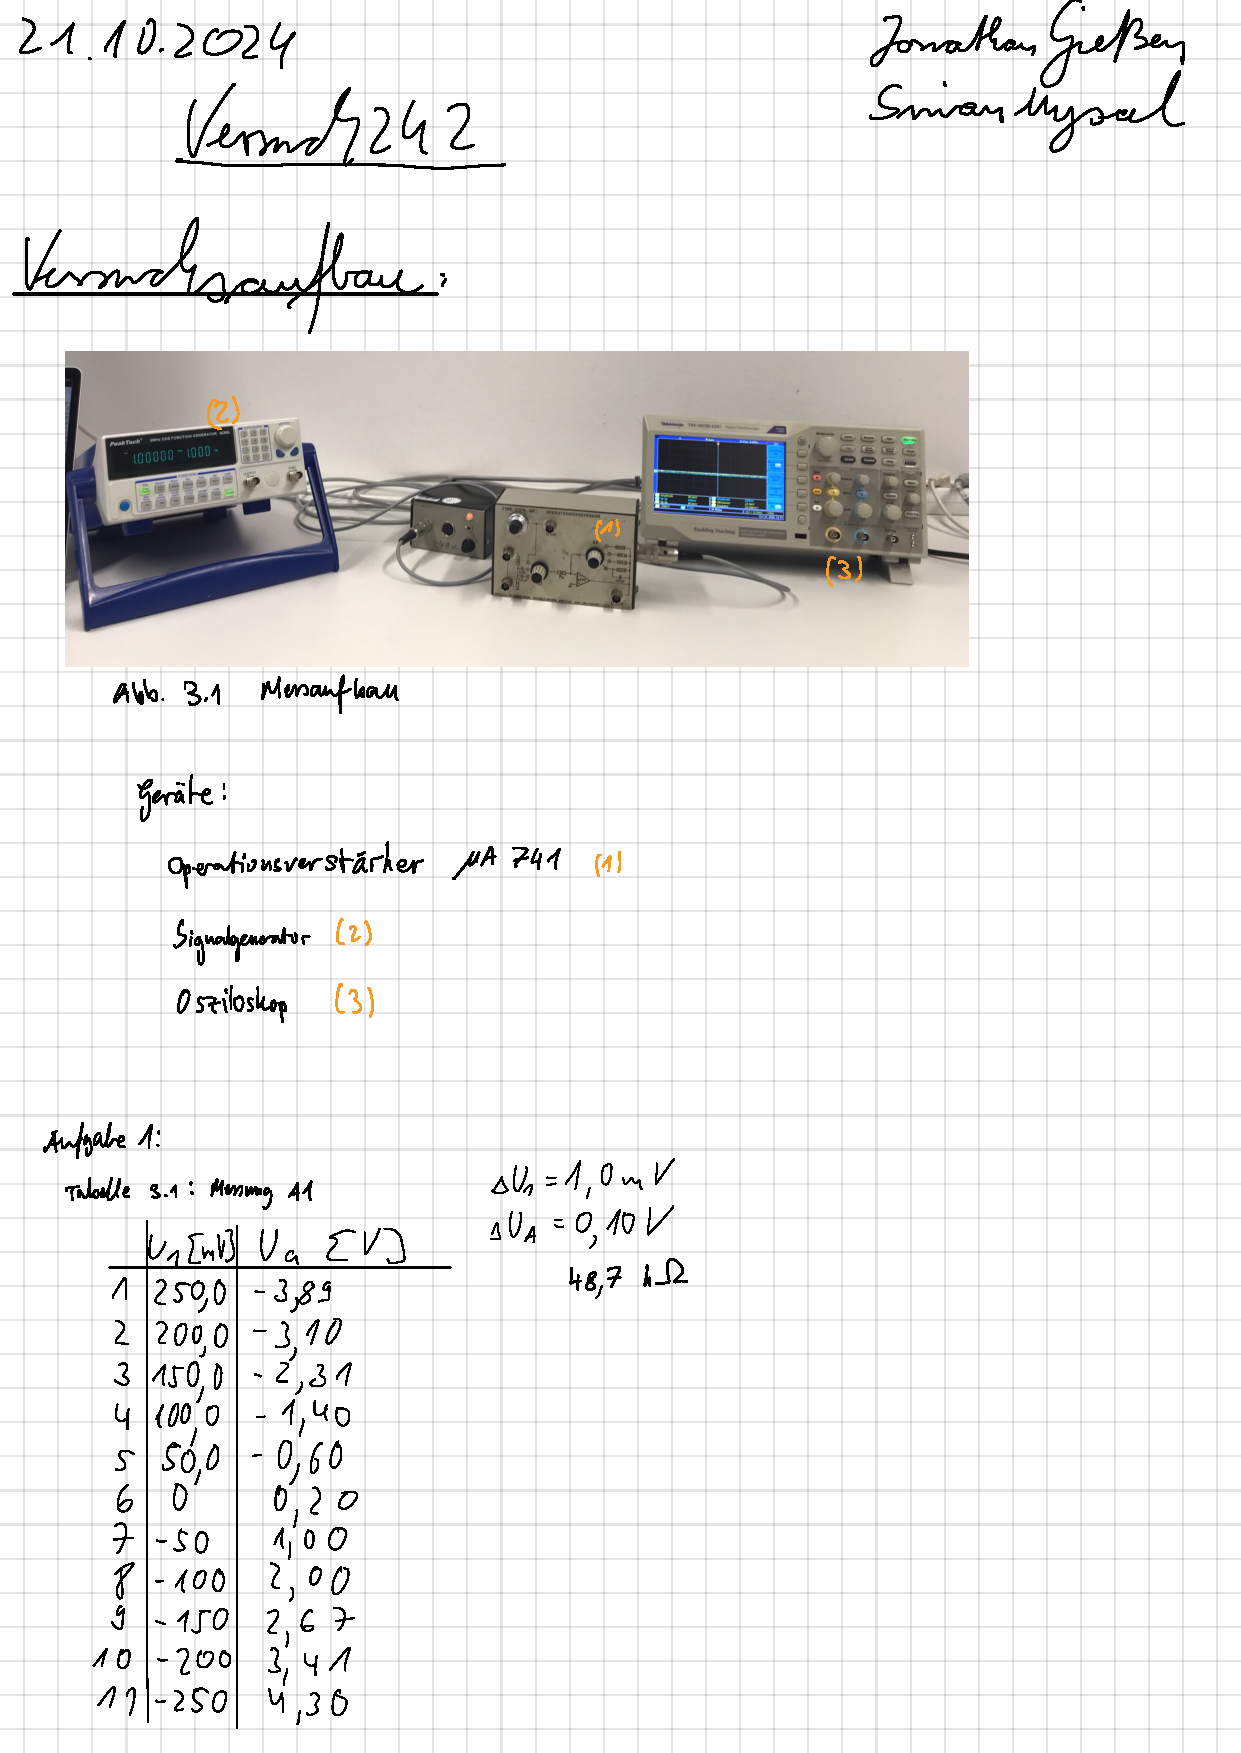
\includepdf[
    pages=-,
    width=\textwidth,
    height=0.92\textheight,
    keepaspectratio,
    pagecommand={\thispagestyle{scrheadings}},
]{../Messprotokoll 22.pdf}

\clearpage


\section{Auswertung}\label{sec:Auswertung}

\subsection{Aufgabe I: Gleich- und Wechselspannungsverstärkung}\label{sec:Aufgabe1}

\subsubsection{Auswertungsmethodik und Fehlerfortpflanzung}

Zur Bestimmung der Betriebsverstärkung $V'$ wird für jede Verstärkerkonfiguration eine gewichtete lineare Regression der Form
\begin{equation}
    U_a(U_1) = m \cdot U_1 + U_{\text{off}}
    \label{eq:lin_reg}
\end{equation}
an die Messwerte angepasst. Da sowohl die Eingangsspannung $U_1$ mit einer Messunsicherheit $\Delta U_1$ als auch die Ausgangsspannung $U_a$ mit $\Delta U_a$ behaftet ist, wird die Unsicherheit $\Delta U_1$ über Gaußsche Fehlerfortpflanzung in eine effektive Gesamtunsicherheit der abhängigen Größe umgerechnet:
\begin{equation}
    \sigma_{\text{eff}} = \sqrt{(\Delta U_a)^2 + (m \cdot \Delta U_1)^2} \,.
    \label{eq:sigma_eff}
\end{equation}

Der Fehler ergibt sich aus der Covarianzmatrix der linearen Regression
\begin{itemize}
    \item \textbf{Gleichspannung (DC):} Die Mess Messunsicherheiten betragen $\Delta U_1 = \SI{1.0}{\milli\volt}$ und $\Delta U_a = \SI{0.10}{\volt}$. Wegen der Invertierung des Signals ($m < 0$) ergibt sich die Betriebsverstärkung zu $V'_{\text{DC}} = -m$ mit $\Delta V'_{\text{DC}} = \Delta m$. Der Achsenabschnitt $U_{\text{off}}$ beschreibt die Ausgangs-Offsetspannung bei $U_1 = \SI{0}{\volt}$.
    \item \textbf{Wechselspannung (AC, $f = \SI{1}{\kilo\hertz}$):} In den Tabellen~\ref{tab:mess_a1_ac274} und~\ref{tab:mess_a1_ac680} wurde auf Kanal~1 der Effektivwert $U_G$ vor dem $1{:}10$-Spannungsteiler mit $\Delta U_G = \SI{3}{\milli\volt}$ gemessen. Für die am Verstärkereingang anliegende Effektivspannung gilt somit:
    \begin{equation}
        U_{1,\text{eff}} = \frac{U_G}{10} \,, \qquad \Delta U_{1,\text{eff}} = \frac{\Delta U_G}{10} = \SI{0.3}{\milli\volt} \,.
    \end{equation}
    Die Ausgangsspannung $U_{a,\text{eff}}$ wurde mit einer Unsicherheit von $\Delta U_{a,\text{eff}} = \SI{10}{\milli\volt}$ bestimmt. Die Steigung liefet $V'_{\text{AC}} = m$.
\end{itemize}

\subsubsection{Beobachtung der Übersteuerung Sättigung bei Gleichspannung}

Bei der Gleichspannungsmessung mit $R_g = \SI{48.7}{\kilo\ohm}$ (Tabelle~\ref{tab:mess_a1_487}) lässt sich ein linearer Zusammenhang $U_a(U_1)$ über das gesamte Messintervall $U_1 \in [\SI{-250}{\milli\volt}, \SI{+250}{\milli\volt}]$ zwischen $U_a = \SI{+4.30}{\volt}$ und $U_a = \SI{-3.89}{\volt}$ erkennen.

Bei der höheren Gegenkopplung $R_g = \SI{274}{\kilo\ohm}$ (Tabelle~\ref{tab:mess_a1_274}) zeigt sich hingegen an den Rändern des Messbereichs die erwartete Sättigung des Operationsverstärkers:
\begin{itemize}
    \item Für positive Eingangsspannungen $U_1 \in \{\SI{150}{\milli\volt}, \SI{200}{\milli\volt}, \SI{250}{\milli\volt}\}$ verharrt die Ausgangsspannung auf einem konstanten Sättigungsplateau von $U_{a,\text{sat}^-} = \SI{-12.70}{\volt}$ bis $\SI{-12.80}{\volt}$.
    \item Für stark negative Eingangsspannungen $U_1 \in \{\SI{-200}{\milli\volt}, \SI{-250}{\milli\volt}\}$ sättigt die Ausgangsspannung bei $U_{a,\text{sat}^+} = \SI{+14.60}{\volt}$ bis $\SI{+14.70}{\volt}$.
\end{itemize}
Die physikalische Ursache hierfür ist die Betriebsspannung des $\mu\text{A}741$ von $U_{\text{CC}} = \pm\SI{15}{\volt}$: Der Operationsverstärker kann lediglich nur knapp unter die Betriebsspannung verstärken. 

\subsubsection{Graphische Darstellung und Ergebnisse zu Aufgabe I}

Abbildung~\ref{fig:aufgabe1_kennlinien} zeigt in Teil~(a) die Gleichspannungskennlinien $U_a(U_1)$ inklusive der Sättigungsbereiche und Residuen sowie in Teil~(b) die Wechselspannungskennlinien $U_{a,\text{eff}}(U_{1,\text{eff}})$ bei $f = \SI{1}{\kilo\hertz}$. 

\begin{figure}[H]
    \centering
    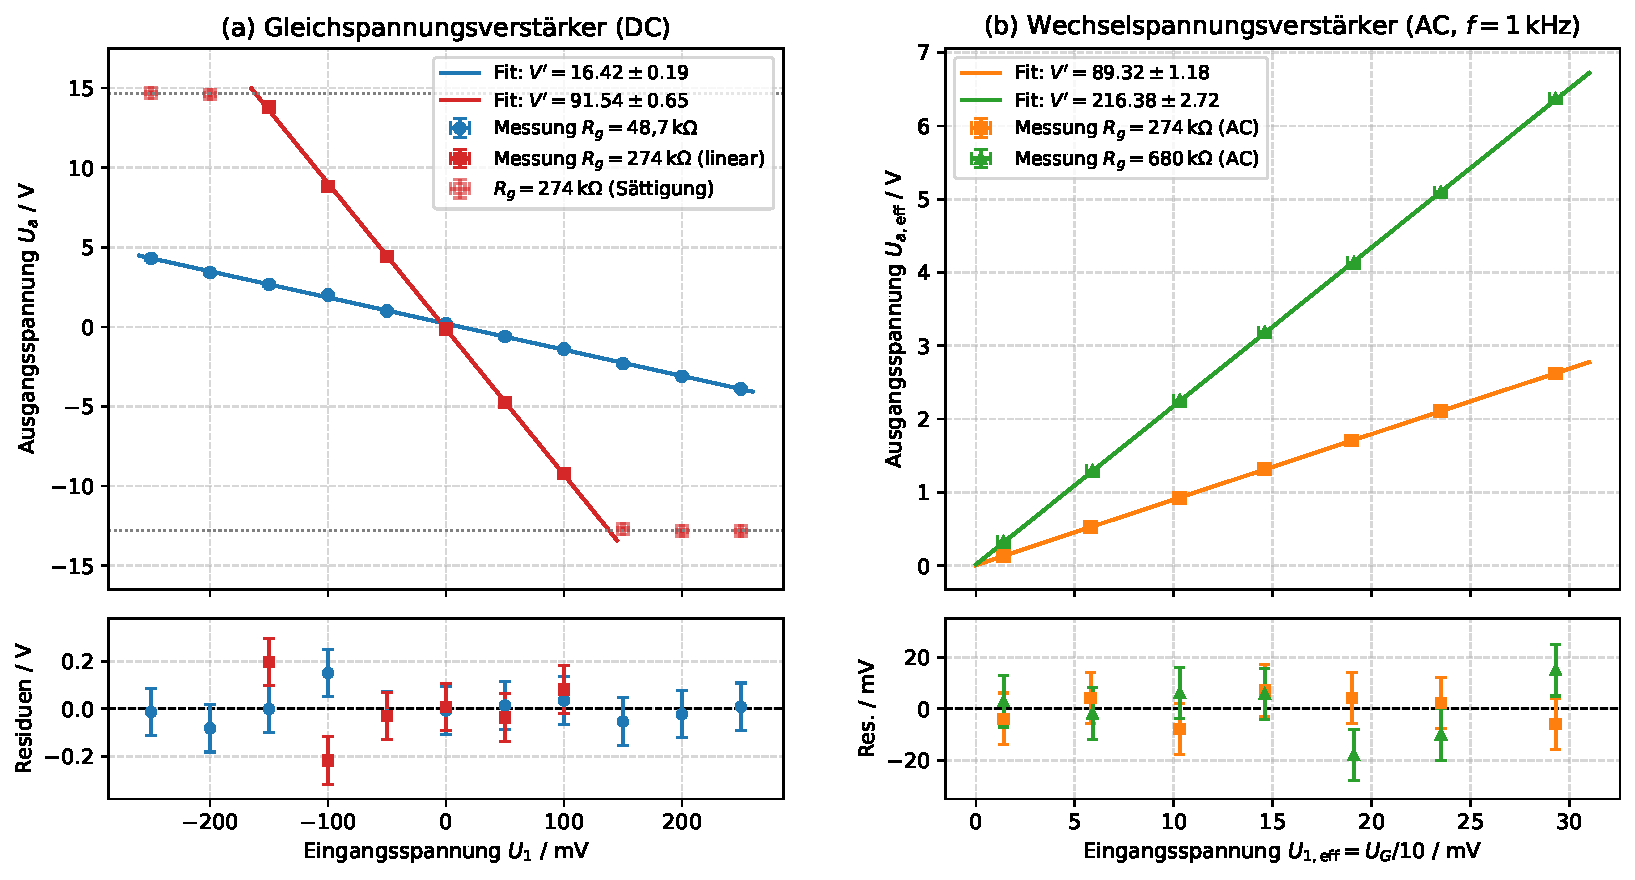
\includegraphics[width=\textwidth]{img/aufgabe1_kennlinien.pdf}
    \caption{Kennlinien der Spannungsverstärkung zu Aufgabe~I: (a) Gleichspannungsverstärker für $R_g = \SI{48.7}{\kilo\ohm}$ und $R_g = \SI{274}{\kilo\ohm}$; (b) Wechselspannungsverstärker bei $f = \SI{1}{\kilo\hertz}$ für $R_g = \SI{274}{\kilo\ohm}$ und $R_g = \SI{680}{\kilo\ohm}$.}
    \label{fig:aufgabe1_kennlinien}
\end{figure}


Die aus den linearen Regressionen gewonnenen Betriebsverstärkungen $V'_{\text{mess}}$, die Offsetspannungen $U_{\text{off}}$ sowie der Vergleich mit den Theoriewerten $V'_{\text{th}} = R_g / R_e$ sind in Tabelle~\ref{tab:ergebnisse_a1} zusammengefasst. Die Sigma-Abweichung der Theorie und der Messwerte lässt sich mit 
\begin{equation}
    z = \frac{|V'_{\text{mess}} - V'_{\text{th}}|}{\sqrt{(\Delta V'_{\text{mess}})^2 + (\Delta V'_{\text{th}})^2}}
\end{equation}
berechnen.

\begin{table}[H]
    \centering
    \caption{Ergebnisse der linearen Regressionen zu Aufgabe~I im Vergleich mit den theoretischen Betriebsverstärkungen $V'_{\text{th}} = R_g / R_e$ ($R_e = \SI{3.0 +- 0.3}{\kilo\ohm}$).}
    \label{tab:ergebnisse_a1}
    \begin{tabular}{llcccc}
        \toprule
        \textbf{Modus} & \textbf{$R_g$} & \textbf{Messwert $V'_{\text{mess}}$} & \textbf{Offset $U_{\text{off}}$} & \textbf{Theorie $V'_{\text{th}}$} & \textbf{Abw. $z$} \\
        \midrule
        DC & $\SI{48.7}{\kilo\ohm}$ & $\num{16.42 +- 0.19}$ & $\SI{0.207 +- 0.031}{\volt}$ & $\num{16.23 +- 2.30}$ & $\num{0.08}\,\sigma$ \\
        DC & $\SI{274}{\kilo\ohm}$ & $\num{91.54 +- 0.65}$ & $\SI{-0.127 +- 0.058}{\volt}$ & $\num{91.33 +- 12.92}$ & $\num{0.02}\,\sigma$ \\
        AC ($\SI{1}{\kilo\hertz}$) & $\SI{274}{\kilo\ohm}$ & $\num{89.32 +- 1.18}$ & $\SI{0.009 +- 0.021}{\volt}$ & $\num{91.33 +- 12.92}$ & $\num{0.16}\,\sigma$ \\
        AC ($\SI{1}{\kilo\hertz}$) & $\SI{680}{\kilo\ohm}$ & $\num{216.38 +- 2.72}$ & $\SI{0.015 +- 0.047}{\volt}$ & $\num{226.67 +- 32.06}$ & $\num{0.32}\,\sigma$ \\
        \bottomrule
    \end{tabular}
\end{table}

\begin{resultbox}[Ergebnis Aufgabe I: Betriebsverstärkungen bei Gleich- und Wechselspannung]
    \small
    \begin{align*}
        V'_{\text{DC}}(\SI{48.7}{\kilo\ohm}) &= \num{16.42 +- 0.19} & &\text{(Theorie: } \num{16.23 +- 2.30},\ \text{Abw.: } \num{0.08}\,\sigma\text{)}\\
        V'_{\text{DC}}(\SI{274}{\kilo\ohm}) &= \num{91.54 +- 0.65} & &\text{(Theorie: } \num{91.33 +- 12.92},\ \text{Abw.: } \num{0.02}\,\sigma\text{)}\\
        V'_{\text{AC}}(\SI{274}{\kilo\ohm}) &= \num{89.32 +- 1.18} & &\text{(Theorie: } \num{91.33 +- 12.92},\ \text{Abw.: } \num{0.16}\,\sigma\text{)}\\
        V'_{\text{AC}}(\SI{680}{\kilo\ohm}) &= \num{216.38 +- 2.72} & &\text{(Theorie: } \num{226.67 +- 32.06},\ \text{Abw.: } \num{0.32}\,\sigma\text{)}
    \end{align*}
\end{resultbox}

% ==============================================================================
% 4.2 AUFGABE II: IMPULSVERSTÄRKUNG
% ==============================================================================
\subsection{Aufgabe II: Impulsverstärkung}\label{sec:Aufgabe3}

In Aufgabe~3 der Durchführung wurde die Übertragung eines Rechtecksignals der Wiederholfrequenz $f_0 = \SI{1}{\kilo\hertz}$ ($T = \SI{1.0}{\milli\second}$) für acht Kombinationen aus Eingangsbeschaltung (Schalter S1) und Gegenkopplung (Schalter S2) am Oszilloskop aufgenommen (Abbildungen~\ref{fig:osz_3_4} bis~\ref{fig:osz_3_11} im Messprotokoll auf den Seiten~4 und~5). Auf den Oszilloskopbildern zeigt die obere Kurve (Kanal~1, gelb) jeweils das eingespeiste Rechtecksignal und die untere Kurve (Kanal~2, blau) das um $\SI{180}{\degree}$ invertierte Ausgangssignal $U_a(t)$.

\subsubsection{Einzelbeschreibung der acht Oszilloskopaufnahmen}

Tabelle~\ref{tab:uebersicht_a3} gibt einen Überblick über die acht Schaltungskonstellationen sowie die jeweils beobachtete Pulsform.

\begin{table}[H]
    \centering
    \caption{Übersicht der acht Oszilloskopaufnahmen zur Impulsverstärkung eines $\SI{1}{\kilo\hertz}$-Rechtecksignals}
    \label{tab:uebersicht_a3}
    \footnotesize
    \setlength{\tabcolsep}{4pt}
    \begin{tabular}{ll>{\raggedright\arraybackslash}p{4.3cm}>{\raggedright\arraybackslash}p{7.4cm}}
        \toprule
        \textbf{Abb.} & \textbf{Schalter} & \textbf{Beschaltung} & \textbf{Beobachtete Ausgangspulsform $U_a(t)$} \\
        \midrule
        \ref{fig:osz_3_4} & S1: 2, S2: 1 & AC ($\SI{22}{\micro\farad}$), $R_g = \SI{680}{\kilo\ohm}$ & Kaum starke Ecken, träger Anstieg. \\
        \addlinespace[3pt]
        \ref{fig:osz_3_5} & S1: 3, S2: 1 & Hochpass ($\SI{47}{\nano\farad}$), $R_g = \SI{680}{\kilo\ohm}$ & "Überdämpfung"\ kaum richtiges Erreichen der maximalen Amplitude \\
        \addlinespace[3pt]
        \ref{fig:osz_3_6} & S1: 2, S2: 2 & AC ($\SI{22}{\micro\farad}$), $R_g = \SI{274}{\kilo\ohm}$ & Deutlich steilerer Anstieg und schärfere Spitzen als bei $\SI{680}{\kilo\ohm}. \Rightarrow$ Geringerer Kopplungswiderstand führt zu ähnlicherem Signal \\
        \addlinespace[3pt]
        \ref{fig:osz_3_7} & S1: 3, S2: 2 & Hochpass ($\SI{47}{\nano\farad}$), $R_g = \SI{274}{\kilo\ohm}$ & Viel weniger Überdämpfung wie bei $\SI{680}{\kilo\ohm}$. Schnellerer Abfall und direkterer Anstieg. \\
        \addlinespace[3pt]
        \ref{fig:osz_3_8} & S1: 2, S2: 3 & AC ($\SI{22}{\micro\farad}$), $R_g = \SI{48.7}{\kilo\ohm}$ & Nahezu ideales, scharfkantiges Rechtecksignal mit steilem Anstieg und flachem Dach. \\
        \addlinespace[3pt]
        \ref{fig:osz_3_9} & S1: 3, S2: 3 & Hochpass ($\SI{47}{\nano\farad}$), $R_g = \SI{48.7}{\kilo\ohm}$ & Differenzierung: extrem scharfe, fast senkrechte Spannungsspitzen an den Flanken und exponentieller Abfall \\
        \addlinespace[3pt]
        \ref{fig:osz_3_10} & S1: 2, S2: 4 & AC ($\SI{22}{\micro\farad}$), $\SI{48.7}{\kilo\ohm} \parallel \SI{560}{\pico\farad}$ & Aktiver Tiefpass: Im Vergleich zu Abb.~\ref{fig:osz_3_8} sind die Flanken und Ecken wieder deutlich exponentiell abgerundet (ähnlich wie Abb.~\ref{fig:osz_3_6}); Dach bleibt flach. \\
        \addlinespace[3pt]
        \ref{fig:osz_3_11} & S1: 3, S2: 4 & Bandpass ($\SI{47}{\nano\farad}$ + $\SI{48.7}{\kilo\ohm} \parallel \SI{560}{\pico\farad}$) & Aktiver Bandpass: Die scharfen Spitzen aus Abb.~\ref{fig:osz_3_9} sind durch den Tiefpass abgerundet und gedämpft, während das Dach exponentiell abfällt. \\
        \bottomrule
    \end{tabular}
\end{table}

\subsubsection{Einfluss der Gegenkopplung und Bedeutung hoher sowie tiefer Frequenzanteile}

Anhand der acht Aufnahmen und des im Messprotokoll (Abbildung~\ref{fig:mess_a2_plot}) dargestellten Frequenzgang lassen sich folgende Schlüsse ziehen:

\begin{enumerate}
    \item \textbf{Auswirkung der Gegenkopplungseinstellungen auf die Impulsform (S1 = 2, Abbildungen~\ref{fig:osz_3_4}, \ref{fig:osz_3_6}, \ref{fig:osz_3_8} und~\ref{fig:osz_3_10}):}
    Mit abnehmendem Rückkopplungswiderstand, also stärkerer Gegenkopplung, steigt die obere Grenzfrequenz. Dadurch Schwingt die Schaltung schneller ein (steilerer Anstieg). 
   
    \item \textbf{Auswirkung des Fehlens hoher oder tiefer Frequenzen:}
    \begin{itemize}
        \item \emph{Fehlen hoher Frequenze: (Tiefpass)} Werden Frequenzen oberhalb von $f_g$ unterdrückt (Abbildungen~\ref{fig:osz_3_4} und~\ref{fig:osz_3_10}), kann die Ausgangsspannung dem abrupten Eingangssprung nicht mehr verzögerungsfrei folgen.
    
        \item \emph{Fehlen tiefer Frequenzen (Hochpass):} Wird der Eingangshochpass $C_{\text{HP}} = \SI{47}{\nano\farad}$ zugeschaltet (S1 = 3, Abbildungen~\ref{fig:osz_3_5}, \ref{fig:osz_3_7}, \ref{fig:osz_3_9} und~\ref{fig:osz_3_11}), werden niedrige Frequenzen unterdrückt. Den Auf- und Entladevorgang des vorgeschalteten Kondensators ist lässt sich in den "Haiflossen" erkennen, (sonst wär es ja wieder ein Rechtecksigmal)
        \item \emph{Fehlen von hohen als auch tiefer Frequenzen (Bandpass, Abbildungen~\ref{fig:osz_3_5} und~\ref{fig:osz_3_11}):} Hier überlagern sich beide Effekte: Der Tiefpass verhindert den steilen Anstieg und kappt die Spitze des Differenzierpeaks, während der Hochpass das Halten der Spannung verhindert. Es entstehen stark gedämpfte, abgerundete Schwingungen auf dem Oszilloskop.
    \end{itemize}
\end{enumerate}

% ==============================================================================
% 5. DISKUSSION UND FAZIT
% ==============================================================================
\section{Diskussion und Fazit}\label{sec:Diskussion}


\begin{enumerate}
    \item \textbf{Verstärkung (Aufgabe~I):}
    Anhand der gemessenen Kennlinien $U_a = f(U_1)$ konnte bestätigt werden, dass die Betriebsverstärkung $V'$ des invertierenden Verstärkers im linearen Arbeitsbereich innerhalb der Messgenauigkeit ausschließlich durch das Verhältnis $R_g / R_e$ der äußeren Beschaltungswiderstände bestimmt wird. Die experimentell ermittelten Verstärkungen $V'_{\text{DC}}(\SI{48.7}{\kilo\ohm}) = \num{16.42 +- 0.19}$, $V'_{\text{DC}}(\SI{274}{\kilo\ohm}) = \num{91.54 +- 0.65}$, $V'_{\text{AC}}(\SI{274}{\kilo\ohm}) = \num{89.32 +- 1.18}$ und $V'_{\text{AC}}(\SI{680}{\kilo\ohm}) = \num{216.38 +- 2.72}$ stimmen mit Abweichungen von lediglich $\num{0.02}\,\sigma$ bis $\num{0.32}\,\sigma$ ausgezeichnet mit den theoretischen Werten ($\num{16.23 +- 2.30}$, $\num{91.33 +- 12.92}$ und $\num{226.67 +- 32.06}$) überein. Auch der direkte Vergleich zwischen Gleich- und Wechselspannungsmessung bei derselben Rückkopplung $R_g = \SI{274}{\kilo\ohm}$ zeigt eine sehr gute Konsistenz ($z = \num{1.65}\,\sigma$). Dass die Wechselspannungsverstärkungen bei $f = \SI{1}{\kilo\hertz}$ geringfügig unter den Gleichspannungswerten liegen, ist bereits auf das Einsetzen des frequezabhängigen Verstärkungsabfalls bei $\SI{1}{\kilo\hertz}$ sowie auf das Teilerverhältnis $\frac{22\,\si{\ohm}}{200\,\si{\ohm}+22\,\si{\ohm}} = \frac{1}{10{,}09}$ des Eingangsteilers zurückzuführen (immerhin 1\%). Bei $R_g = \SI{274}{\kilo\ohm}$ im Gleichspannungsbetrieb konnte zudem die Stättigung der Verstärkungskurve durch die Betriebsspannung ($\pm\SI{15}{\volt}$) nachgewiesen werden. 

    \item \textbf{Auswirkung auf die Impulsform (Aufgabe~II):}
    Der im Messprotokoll (Abbildung~\ref{fig:mess_a2_plot}) aufgexnommene Frequenzgang zwischen $\SI{100}{\hertz}$ und $\SI{300}{\kilo\hertz}$ bestätigte den fundamentalen Zusammenhang zwischen Gegenkopplung und Bandbreite: Eine Reduktion von $R_g$ senkt die Niederfrequenzverstärkung $V'_0$, erweitert jedoch im gleichen Maße die Bandbreite $f_g$. (Für den Praktischen Fall gut zu wissen). 
    Fehlerabwichungen

    Die Oszilloskopaufnahmen eines $\SI{1}{\kilo\hertz}$-Rechtecksignals demonstrierten den Zusammenhang zwischen Frequenzgang und Zeitbereich: Während eine hohe Bandbreite ($R_g = \SI{48.7}{\kilo\ohm}$) eine nahezu verzerrungsfreie Rechteckübertragung erlaubt, führt das Fehlen hoher Frequenzen (kleines $f_g$ bei großem $R_g$ oder aktivem Tiefpass) zu einer Lähmung der Anstiege und Abflachungen (Integrierwirkung\footnotemark[1]), und das Fehlen tiefer Frequenzen durch den Eingangshochpass zu einem exponentiellen Einbruch des Impulsdachs (Differenzierwirkung\footnotemark[1])
\end{enumerate}

\footnotetext[1]{Versuch 241 - Hier wird beschreiben die Integrier und Differenzierwirkung des Hoch- und Tiefpass' \cite{PAPskript}}

\clearpage

\listoffigures

\listoftables

\begin{thebibliography}{5}
    \bibitem{PAPskript} Dr. J. Wagner, \emph{Physikalisches Anfängerpraktikum -- Praktikum IIb, Versuch 242: Spannungsverstärkung mit dem Operationsverstärker}, Universität Heidelberg, Stand 11/2025.
    \bibitem{ilberg1988physikalisches} W. Ilberg, M. Krötzsch, \emph{Physikalisches Praktikum für Anfänger}, BSB B. G. Teubner Verlagsgesellschaft, Leipzig (1985).
    \bibitem{tietze} U. Tietze, Ch. Schenk, E. Gamm, \emph{Halbleiter-Schaltungstechnik}, Springer-Verlag, Berlin/Heidelberg.
\end{thebibliography}

\appendix

\section{Anhang: Code}



    
    \begin{tcolorbox}[breakable, size=fbox, boxrule=1pt, pad at break*=1mm,colback=cellbackground, colframe=cellborder]
\prompt{In}{incolor}{9}{\boxspacing}
\begin{Verbatim}[commandchars=\\\{\}]
\PY{k+kn}{import}\PY{+w}{ }\PY{n+nn}{numpy}\PY{+w}{ }\PY{k}{as}\PY{+w}{ }\PY{n+nn}{np}
\PY{k+kn}{import}\PY{+w}{ }\PY{n+nn}{matplotlib}\PY{n+nn}{.}\PY{n+nn}{pyplot}\PY{+w}{ }\PY{k}{as}\PY{+w}{ }\PY{n+nn}{plt}
\PY{k+kn}{from}\PY{+w}{ }\PY{n+nn}{scipy}\PY{n+nn}{.}\PY{n+nn}{optimize}\PY{+w}{ }\PY{k+kn}{import} \PY{n}{curve\PYZus{}fit}
\end{Verbatim}
\end{tcolorbox}

    Messung A1.1

    \begin{tcolorbox}[breakable, size=fbox, boxrule=1pt, pad at break*=1mm,colback=cellbackground, colframe=cellborder]
\prompt{In}{incolor}{10}{\boxspacing}
\begin{Verbatim}[commandchars=\\\{\}]
\PY{n}{R\PYZus{}e} \PY{o}{=} \PY{l+m+mf}{3.0e3}
\PY{n}{dR\PYZus{}e} \PY{o}{=} \PY{l+m+mf}{0.10} \PY{o}{*} \PY{n}{R\PYZus{}e}

\PY{c+c1}{\PYZsh{} DC}
\PY{n}{U1\PYZus{}dc} \PY{o}{=} \PY{n}{np}\PY{o}{.}\PY{n}{array}\PY{p}{(}\PY{p}{[}\PY{l+m+mi}{250}\PY{p}{,} \PY{l+m+mi}{200}\PY{p}{,} \PY{l+m+mi}{150}\PY{p}{,} \PY{l+m+mi}{100}\PY{p}{,} \PY{l+m+mi}{50}\PY{p}{,} \PY{l+m+mi}{0}\PY{p}{,} \PY{o}{\PYZhy{}}\PY{l+m+mi}{50}\PY{p}{,} \PY{o}{\PYZhy{}}\PY{l+m+mi}{100}\PY{p}{,} \PY{o}{\PYZhy{}}\PY{l+m+mi}{150}\PY{p}{,} \PY{o}{\PYZhy{}}\PY{l+m+mi}{200}\PY{p}{,} \PY{o}{\PYZhy{}}\PY{l+m+mi}{250}\PY{p}{]}\PY{p}{)} \PY{o}{*} \PY{l+m+mf}{1e\PYZhy{}3}
\PY{n}{dU1\PYZus{}dc} \PY{o}{=} \PY{l+m+mf}{1.0e\PYZhy{}3}

\PY{n}{Ua\PYZus{}dc\PYZus{}487} \PY{o}{=} \PY{n}{np}\PY{o}{.}\PY{n}{array}\PY{p}{(}\PY{p}{[}\PY{o}{\PYZhy{}}\PY{l+m+mf}{3.89}\PY{p}{,} \PY{o}{\PYZhy{}}\PY{l+m+mf}{3.10}\PY{p}{,} \PY{o}{\PYZhy{}}\PY{l+m+mf}{2.31}\PY{p}{,} \PY{o}{\PYZhy{}}\PY{l+m+mf}{1.40}\PY{p}{,} \PY{o}{\PYZhy{}}\PY{l+m+mf}{0.60}\PY{p}{,} \PY{l+m+mf}{0.20}\PY{p}{,} \PY{l+m+mf}{1.00}\PY{p}{,} \PY{l+m+mf}{2.00}\PY{p}{,} \PY{l+m+mf}{2.67}\PY{p}{,} \PY{l+m+mf}{3.41}\PY{p}{,} \PY{l+m+mf}{4.30}\PY{p}{]}\PY{p}{)}
\PY{n}{Ua\PYZus{}dc\PYZus{}274} \PY{o}{=} \PY{n}{np}\PY{o}{.}\PY{n}{array}\PY{p}{(}\PY{p}{[}\PY{o}{\PYZhy{}}\PY{l+m+mf}{12.80}\PY{p}{,} \PY{o}{\PYZhy{}}\PY{l+m+mf}{12.80}\PY{p}{,} \PY{o}{\PYZhy{}}\PY{l+m+mf}{12.70}\PY{p}{,} \PY{o}{\PYZhy{}}\PY{l+m+mf}{9.20}\PY{p}{,} \PY{o}{\PYZhy{}}\PY{l+m+mf}{4.74}\PY{p}{,} \PY{o}{\PYZhy{}}\PY{l+m+mf}{0.12}\PY{p}{,} \PY{l+m+mf}{4.42}\PY{p}{,} \PY{l+m+mf}{8.81}\PY{p}{,} \PY{l+m+mf}{13.80}\PY{p}{,} \PY{l+m+mf}{14.60}\PY{p}{,} \PY{l+m+mf}{14.70}\PY{p}{]}\PY{p}{)}
\PY{n}{dUa\PYZus{}dc} \PY{o}{=} \PY{l+m+mf}{0.10}

\PY{c+c1}{\PYZsh{} AC (1 kHz)}
\PY{n}{Uss\PYZus{}ac} \PY{o}{=} \PY{n}{np}\PY{o}{.}\PY{n}{array}\PY{p}{(}\PY{p}{[}\PY{l+m+mi}{50}\PY{p}{,} \PY{l+m+mi}{200}\PY{p}{,} \PY{l+m+mi}{350}\PY{p}{,} \PY{l+m+mi}{500}\PY{p}{,} \PY{l+m+mi}{650}\PY{p}{,} \PY{l+m+mi}{800}\PY{p}{,} \PY{l+m+mi}{1000}\PY{p}{]}\PY{p}{)} \PY{o}{*} \PY{l+m+mf}{1e\PYZhy{}3}

\PY{n}{UG\PYZus{}ac\PYZus{}274} \PY{o}{=} \PY{n}{np}\PY{o}{.}\PY{n}{array}\PY{p}{(}\PY{p}{[}\PY{l+m+mi}{14}\PY{p}{,} \PY{l+m+mi}{58}\PY{p}{,} \PY{l+m+mi}{103}\PY{p}{,} \PY{l+m+mi}{146}\PY{p}{,} \PY{l+m+mi}{190}\PY{p}{,} \PY{l+m+mi}{235}\PY{p}{,} \PY{l+m+mi}{293}\PY{p}{]}\PY{p}{)} \PY{o}{*} \PY{l+m+mf}{1e\PYZhy{}3}
\PY{n}{U1\PYZus{}ac\PYZus{}274} \PY{o}{=} \PY{n}{UG\PYZus{}ac\PYZus{}274} \PY{o}{/} \PY{l+m+mi}{10}
\PY{n}{Ua\PYZus{}ac\PYZus{}274} \PY{o}{=} \PY{n}{np}\PY{o}{.}\PY{n}{array}\PY{p}{(}\PY{p}{[}\PY{l+m+mi}{130}\PY{p}{,} \PY{l+m+mi}{531}\PY{p}{,} \PY{l+m+mi}{921}\PY{p}{,} \PY{l+m+mi}{1320}\PY{p}{,} \PY{l+m+mi}{1710}\PY{p}{,} \PY{l+m+mi}{2110}\PY{p}{,} \PY{l+m+mi}{2620}\PY{p}{]}\PY{p}{)} \PY{o}{*} \PY{l+m+mf}{1e\PYZhy{}3}

\PY{n}{UG\PYZus{}ac\PYZus{}680} \PY{o}{=} \PY{n}{np}\PY{o}{.}\PY{n}{array}\PY{p}{(}\PY{p}{[}\PY{l+m+mi}{14}\PY{p}{,} \PY{l+m+mi}{59}\PY{p}{,} \PY{l+m+mi}{103}\PY{p}{,} \PY{l+m+mi}{146}\PY{p}{,} \PY{l+m+mi}{191}\PY{p}{,} \PY{l+m+mi}{235}\PY{p}{,} \PY{l+m+mi}{293}\PY{p}{]}\PY{p}{)} \PY{o}{*} \PY{l+m+mf}{1e\PYZhy{}3}
\PY{n}{U1\PYZus{}ac\PYZus{}680} \PY{o}{=} \PY{n}{UG\PYZus{}ac\PYZus{}680} \PY{o}{/} \PY{l+m+mi}{10}
\PY{n}{Ua\PYZus{}ac\PYZus{}680} \PY{o}{=} \PY{n}{np}\PY{o}{.}\PY{n}{array}\PY{p}{(}\PY{p}{[}\PY{l+m+mi}{321}\PY{p}{,} \PY{l+m+mi}{1290}\PY{p}{,} \PY{l+m+mi}{2250}\PY{p}{,} \PY{l+m+mi}{3180}\PY{p}{,} \PY{l+m+mi}{4130}\PY{p}{,} \PY{l+m+mi}{5090}\PY{p}{,} \PY{l+m+mi}{6370}\PY{p}{]}\PY{p}{)} \PY{o}{*} \PY{l+m+mf}{1e\PYZhy{}3}

\PY{n}{dUG\PYZus{}ac} \PY{o}{=} \PY{l+m+mf}{3.0e\PYZhy{}3}
\PY{n}{dU1\PYZus{}ac} \PY{o}{=} \PY{n}{dUG\PYZus{}ac} \PY{o}{/} \PY{l+m+mi}{10}
\PY{n}{dUa\PYZus{}ac} \PY{o}{=} \PY{l+m+mf}{10.0e\PYZhy{}3}
\end{Verbatim}
\end{tcolorbox}

    A1 berechenen

    \begin{tcolorbox}[breakable, size=fbox, boxrule=1pt, pad at break*=1mm,colback=cellbackground, colframe=cellborder]
\prompt{In}{incolor}{11}{\boxspacing}
\begin{Verbatim}[commandchars=\\\{\}]
\PY{k}{def}\PY{+w}{ }\PY{n+nf}{lin\PYZus{}model}\PY{p}{(}\PY{n}{x}\PY{p}{,} \PY{n}{m}\PY{p}{,} \PY{n}{b}\PY{p}{)}\PY{p}{:}
    \PY{k}{return} \PY{n}{m} \PY{o}{*} \PY{n}{x} \PY{o}{+} \PY{n}{b}

\PY{k}{def}\PY{+w}{ }\PY{n+nf}{fit\PYZus{}linear}\PY{p}{(}\PY{n}{x}\PY{p}{,} \PY{n}{y}\PY{p}{,} \PY{n}{dx}\PY{p}{,} \PY{n}{dy}\PY{p}{)}\PY{p}{:}
    \PY{n}{popt}\PY{p}{,} \PY{n}{pcov} \PY{o}{=} \PY{n}{curve\PYZus{}fit}\PY{p}{(}\PY{n}{lin\PYZus{}model}\PY{p}{,} \PY{n}{x}\PY{p}{,} \PY{n}{y}\PY{p}{,} \PY{n}{sigma}\PY{o}{=}\PY{n}{np}\PY{o}{.}\PY{n}{full\PYZus{}like}\PY{p}{(}\PY{n}{y}\PY{p}{,} \PY{n}{dy}\PY{p}{)}\PY{p}{,} \PY{n}{absolute\PYZus{}sigma}\PY{o}{=}\PY{k+kc}{True}\PY{p}{)}
    \PY{k}{for} \PY{n}{\PYZus{}} \PY{o+ow}{in} \PY{n+nb}{range}\PY{p}{(}\PY{l+m+mi}{3}\PY{p}{)}\PY{p}{:}
        \PY{n}{dy\PYZus{}eff} \PY{o}{=} \PY{n}{np}\PY{o}{.}\PY{n}{sqrt}\PY{p}{(}\PY{n}{dy}\PY{o}{*}\PY{o}{*}\PY{l+m+mi}{2} \PY{o}{+} \PY{p}{(}\PY{n}{popt}\PY{p}{[}\PY{l+m+mi}{0}\PY{p}{]} \PY{o}{*} \PY{n}{dx}\PY{p}{)}\PY{o}{*}\PY{o}{*}\PY{l+m+mi}{2}\PY{p}{)}
        \PY{n}{popt}\PY{p}{,} \PY{n}{pcov} \PY{o}{=} \PY{n}{curve\PYZus{}fit}\PY{p}{(}\PY{n}{lin\PYZus{}model}\PY{p}{,} \PY{n}{x}\PY{p}{,} \PY{n}{y}\PY{p}{,} \PY{n}{sigma}\PY{o}{=}\PY{n}{dy\PYZus{}eff}\PY{p}{,} \PY{n}{absolute\PYZus{}sigma}\PY{o}{=}\PY{k+kc}{True}\PY{p}{)}
    \PY{n}{perr} \PY{o}{=} \PY{n}{np}\PY{o}{.}\PY{n}{sqrt}\PY{p}{(}\PY{n}{np}\PY{o}{.}\PY{n}{diag}\PY{p}{(}\PY{n}{pcov}\PY{p}{)}\PY{p}{)}
    \PY{k}{return} \PY{n}{popt}\PY{p}{,} \PY{n}{perr}

\PY{n}{popt\PYZus{}dc487}\PY{p}{,} \PY{n}{perr\PYZus{}dc487} \PY{o}{=} \PY{n}{fit\PYZus{}linear}\PY{p}{(}\PY{n}{U1\PYZus{}dc}\PY{p}{,} \PY{n}{Ua\PYZus{}dc\PYZus{}487}\PY{p}{,} \PY{n}{dU1\PYZus{}dc}\PY{p}{,} \PY{n}{dUa\PYZus{}dc}\PY{p}{)}

\PY{n}{lin\PYZus{}mask\PYZus{}274} \PY{o}{=} \PY{n}{np}\PY{o}{.}\PY{n}{zeros}\PY{p}{(}\PY{n+nb}{len}\PY{p}{(}\PY{n}{U1\PYZus{}dc}\PY{p}{)}\PY{p}{,} \PY{n}{dtype}\PY{o}{=}\PY{n+nb}{bool}\PY{p}{)}
\PY{n}{lin\PYZus{}mask\PYZus{}274}\PY{p}{[}\PY{l+m+mi}{3}\PY{p}{:}\PY{l+m+mi}{9}\PY{p}{]} \PY{o}{=} \PY{k+kc}{True}
\PY{n}{popt\PYZus{}dc274}\PY{p}{,} \PY{n}{perr\PYZus{}dc274} \PY{o}{=} \PY{n}{fit\PYZus{}linear}\PY{p}{(}\PY{n}{U1\PYZus{}dc}\PY{p}{[}\PY{n}{lin\PYZus{}mask\PYZus{}274}\PY{p}{]}\PY{p}{,} \PY{n}{Ua\PYZus{}dc\PYZus{}274}\PY{p}{[}\PY{n}{lin\PYZus{}mask\PYZus{}274}\PY{p}{]}\PY{p}{,} \PY{n}{dU1\PYZus{}dc}\PY{p}{,} \PY{n}{dUa\PYZus{}dc}\PY{p}{)}

\PY{n}{popt\PYZus{}ac274}\PY{p}{,} \PY{n}{perr\PYZus{}ac274} \PY{o}{=} \PY{n}{fit\PYZus{}linear}\PY{p}{(}\PY{n}{U1\PYZus{}ac\PYZus{}274}\PY{p}{,} \PY{n}{Ua\PYZus{}ac\PYZus{}274}\PY{p}{,} \PY{n}{dU1\PYZus{}ac}\PY{p}{,} \PY{n}{dUa\PYZus{}ac}\PY{p}{)}
\PY{n}{popt\PYZus{}ac680}\PY{p}{,} \PY{n}{perr\PYZus{}ac680} \PY{o}{=} \PY{n}{fit\PYZus{}linear}\PY{p}{(}\PY{n}{U1\PYZus{}ac\PYZus{}680}\PY{p}{,} \PY{n}{Ua\PYZus{}ac\PYZus{}680}\PY{p}{,} \PY{n}{dU1\PYZus{}ac}\PY{p}{,} \PY{n}{dUa\PYZus{}ac}\PY{p}{)}

\PY{k}{for} \PY{n}{label}\PY{p}{,} \PY{n}{Rg}\PY{p}{,} \PY{n}{V\PYZus{}m}\PY{p}{,} \PY{n}{dV\PYZus{}m}\PY{p}{,} \PY{n}{b}\PY{p}{,} \PY{n}{db} \PY{o+ow}{in} \PY{p}{[}
    \PY{p}{(}\PY{l+s+s1}{\PYZsq{}}\PY{l+s+s1}{DC 48.7k}\PY{l+s+s1}{\PYZsq{}}\PY{p}{,} \PY{l+m+mf}{48.7e3}\PY{p}{,} \PY{o}{\PYZhy{}}\PY{n}{popt\PYZus{}dc487}\PY{p}{[}\PY{l+m+mi}{0}\PY{p}{]}\PY{p}{,} \PY{n}{perr\PYZus{}dc487}\PY{p}{[}\PY{l+m+mi}{0}\PY{p}{]}\PY{p}{,} \PY{n}{popt\PYZus{}dc487}\PY{p}{[}\PY{l+m+mi}{1}\PY{p}{]}\PY{p}{,} \PY{n}{perr\PYZus{}dc487}\PY{p}{[}\PY{l+m+mi}{1}\PY{p}{]}\PY{p}{)}\PY{p}{,}
    \PY{p}{(}\PY{l+s+s1}{\PYZsq{}}\PY{l+s+s1}{DC 274k }\PY{l+s+s1}{\PYZsq{}}\PY{p}{,} \PY{l+m+mf}{274.0e3}\PY{p}{,} \PY{o}{\PYZhy{}}\PY{n}{popt\PYZus{}dc274}\PY{p}{[}\PY{l+m+mi}{0}\PY{p}{]}\PY{p}{,} \PY{n}{perr\PYZus{}dc274}\PY{p}{[}\PY{l+m+mi}{0}\PY{p}{]}\PY{p}{,} \PY{n}{popt\PYZus{}dc274}\PY{p}{[}\PY{l+m+mi}{1}\PY{p}{]}\PY{p}{,} \PY{n}{perr\PYZus{}dc274}\PY{p}{[}\PY{l+m+mi}{1}\PY{p}{]}\PY{p}{)}\PY{p}{,}
    \PY{p}{(}\PY{l+s+s1}{\PYZsq{}}\PY{l+s+s1}{AC 274k }\PY{l+s+s1}{\PYZsq{}}\PY{p}{,} \PY{l+m+mf}{274.0e3}\PY{p}{,}  \PY{n}{popt\PYZus{}ac274}\PY{p}{[}\PY{l+m+mi}{0}\PY{p}{]}\PY{p}{,} \PY{n}{perr\PYZus{}ac274}\PY{p}{[}\PY{l+m+mi}{0}\PY{p}{]}\PY{p}{,} \PY{n}{popt\PYZus{}ac274}\PY{p}{[}\PY{l+m+mi}{1}\PY{p}{]}\PY{p}{,} \PY{n}{perr\PYZus{}ac274}\PY{p}{[}\PY{l+m+mi}{1}\PY{p}{]}\PY{p}{)}\PY{p}{,}
    \PY{p}{(}\PY{l+s+s1}{\PYZsq{}}\PY{l+s+s1}{AC 680k }\PY{l+s+s1}{\PYZsq{}}\PY{p}{,} \PY{l+m+mf}{680.0e3}\PY{p}{,}  \PY{n}{popt\PYZus{}ac680}\PY{p}{[}\PY{l+m+mi}{0}\PY{p}{]}\PY{p}{,} \PY{n}{perr\PYZus{}ac680}\PY{p}{[}\PY{l+m+mi}{0}\PY{p}{]}\PY{p}{,} \PY{n}{popt\PYZus{}ac680}\PY{p}{[}\PY{l+m+mi}{1}\PY{p}{]}\PY{p}{,} \PY{n}{perr\PYZus{}ac680}\PY{p}{[}\PY{l+m+mi}{1}\PY{p}{]}\PY{p}{)}\PY{p}{,}
\PY{p}{]}\PY{p}{:}
    \PY{n}{V\PYZus{}th} \PY{o}{=} \PY{n}{Rg} \PY{o}{/} \PY{n}{R\PYZus{}e}
    \PY{n}{dV\PYZus{}th} \PY{o}{=} \PY{n}{V\PYZus{}th} \PY{o}{*} \PY{n}{np}\PY{o}{.}\PY{n}{sqrt}\PY{p}{(}\PY{l+m+mf}{0.10}\PY{o}{*}\PY{o}{*}\PY{l+m+mi}{2} \PY{o}{+} \PY{l+m+mf}{0.10}\PY{o}{*}\PY{o}{*}\PY{l+m+mi}{2}\PY{p}{)}
    \PY{n}{z} \PY{o}{=} \PY{n+nb}{abs}\PY{p}{(}\PY{n}{V\PYZus{}m} \PY{o}{\PYZhy{}} \PY{n}{V\PYZus{}th}\PY{p}{)} \PY{o}{/} \PY{n}{np}\PY{o}{.}\PY{n}{sqrt}\PY{p}{(}\PY{n}{dV\PYZus{}m}\PY{o}{*}\PY{o}{*}\PY{l+m+mi}{2} \PY{o}{+} \PY{n}{dV\PYZus{}th}\PY{o}{*}\PY{o}{*}\PY{l+m+mi}{2}\PY{p}{)}
    \PY{n+nb}{print}\PY{p}{(}\PY{l+s+sa}{f}\PY{l+s+s1}{\PYZsq{}}\PY{l+s+si}{\PYZob{}}\PY{n}{label}\PY{l+s+si}{\PYZcb{}}\PY{l+s+s1}{: V = }\PY{l+s+si}{\PYZob{}}\PY{n}{V\PYZus{}m}\PY{l+s+si}{:}\PY{l+s+s1}{.2f}\PY{l+s+si}{\PYZcb{}}\PY{l+s+s1}{ +\PYZhy{} }\PY{l+s+si}{\PYZob{}}\PY{n}{dV\PYZus{}m}\PY{l+s+si}{:}\PY{l+s+s1}{.2f}\PY{l+s+si}{\PYZcb{}}\PY{l+s+s1}{, U\PYZus{}off = }\PY{l+s+si}{\PYZob{}}\PY{n}{b}\PY{l+s+si}{:}\PY{l+s+s1}{.3f}\PY{l+s+si}{\PYZcb{}}\PY{l+s+s1}{ +\PYZhy{} }\PY{l+s+si}{\PYZob{}}\PY{n}{db}\PY{l+s+si}{:}\PY{l+s+s1}{.3f}\PY{l+s+si}{\PYZcb{}}\PY{l+s+s1}{, V\PYZus{}th = }\PY{l+s+si}{\PYZob{}}\PY{n}{V\PYZus{}th}\PY{l+s+si}{:}\PY{l+s+s1}{.2f}\PY{l+s+si}{\PYZcb{}}\PY{l+s+s1}{ +\PYZhy{} }\PY{l+s+si}{\PYZob{}}\PY{n}{dV\PYZus{}th}\PY{l+s+si}{:}\PY{l+s+s1}{.2f}\PY{l+s+si}{\PYZcb{}}\PY{l+s+s1}{, z = }\PY{l+s+si}{\PYZob{}}\PY{n}{z}\PY{l+s+si}{:}\PY{l+s+s1}{.2f}\PY{l+s+si}{\PYZcb{}}\PY{l+s+s1}{\PYZsq{}}\PY{p}{)}
\end{Verbatim}
\end{tcolorbox}

    \begin{Verbatim}[commandchars=\\\{\}]
DC 48.7k: V = 16.42 +- 0.19, U\_off = 0.207 +- 0.031, V\_th = 16.23 +- 2.30, z =
0.08
DC 274k : V = 91.54 +- 0.65, U\_off = -0.127 +- 0.058, V\_th = 91.33 +- 12.92, z =
0.02
AC 274k : V = 89.32 +- 1.18, U\_off = 0.009 +- 0.021, V\_th = 91.33 +- 12.92, z =
0.16
AC 680k : V = 216.38 +- 2.72, U\_off = 0.015 +- 0.047, V\_th = 226.67 +- 32.06, z
= 0.32
    \end{Verbatim}

    \begin{tcolorbox}[breakable, size=fbox, boxrule=1pt, pad at break*=1mm,colback=cellbackground, colframe=cellborder]
\prompt{In}{incolor}{ }{\boxspacing}
\begin{Verbatim}[commandchars=\\\{\}]
\PY{n}{fig} \PY{o}{=} \PY{n}{plt}\PY{o}{.}\PY{n}{figure}\PY{p}{(}\PY{n}{figsize}\PY{o}{=}\PY{p}{(}\PY{l+m+mi}{13}\PY{p}{,} \PY{l+m+mf}{6.5}\PY{p}{)}\PY{p}{)}
\PY{n}{gs} \PY{o}{=} \PY{n}{fig}\PY{o}{.}\PY{n}{add\PYZus{}gridspec}\PY{p}{(}\PY{l+m+mi}{2}\PY{p}{,} \PY{l+m+mi}{2}\PY{p}{,} \PY{n}{height\PYZus{}ratios}\PY{o}{=}\PY{p}{[}\PY{l+m+mi}{3}\PY{p}{,} \PY{l+m+mi}{1}\PY{p}{]}\PY{p}{,} \PY{n}{hspace}\PY{o}{=}\PY{l+m+mf}{0.08}\PY{p}{,} \PY{n}{wspace}\PY{o}{=}\PY{l+m+mf}{0.24}\PY{p}{)}

\PY{n}{ax\PYZus{}dc} \PY{o}{=} \PY{n}{fig}\PY{o}{.}\PY{n}{add\PYZus{}subplot}\PY{p}{(}\PY{n}{gs}\PY{p}{[}\PY{l+m+mi}{0}\PY{p}{,} \PY{l+m+mi}{0}\PY{p}{]}\PY{p}{)}
\PY{n}{ax\PYZus{}dc\PYZus{}res} \PY{o}{=} \PY{n}{fig}\PY{o}{.}\PY{n}{add\PYZus{}subplot}\PY{p}{(}\PY{n}{gs}\PY{p}{[}\PY{l+m+mi}{1}\PY{p}{,} \PY{l+m+mi}{0}\PY{p}{]}\PY{p}{,} \PY{n}{sharex}\PY{o}{=}\PY{n}{ax\PYZus{}dc}\PY{p}{)}
\PY{n}{ax\PYZus{}ac} \PY{o}{=} \PY{n}{fig}\PY{o}{.}\PY{n}{add\PYZus{}subplot}\PY{p}{(}\PY{n}{gs}\PY{p}{[}\PY{l+m+mi}{0}\PY{p}{,} \PY{l+m+mi}{1}\PY{p}{]}\PY{p}{)}
\PY{n}{ax\PYZus{}ac\PYZus{}res} \PY{o}{=} \PY{n}{fig}\PY{o}{.}\PY{n}{add\PYZus{}subplot}\PY{p}{(}\PY{n}{gs}\PY{p}{[}\PY{l+m+mi}{1}\PY{p}{,} \PY{l+m+mi}{1}\PY{p}{]}\PY{p}{,} \PY{n}{sharex}\PY{o}{=}\PY{n}{ax\PYZus{}ac}\PY{p}{)}

\PY{n}{x\PYZus{}dc} \PY{o}{=} \PY{n}{np}\PY{o}{.}\PY{n}{linspace}\PY{p}{(}\PY{o}{\PYZhy{}}\PY{l+m+mi}{260}\PY{p}{,} \PY{l+m+mi}{260}\PY{p}{,} \PY{l+m+mi}{200}\PY{p}{)}
\PY{n}{ax\PYZus{}dc}\PY{o}{.}\PY{n}{errorbar}\PY{p}{(}\PY{n}{U1\PYZus{}dc} \PY{o}{*} \PY{l+m+mf}{1e3}\PY{p}{,} \PY{n}{Ua\PYZus{}dc\PYZus{}487}\PY{p}{,} \PY{n}{xerr}\PY{o}{=}\PY{n}{dU1\PYZus{}dc} \PY{o}{*} \PY{l+m+mf}{1e3}\PY{p}{,} \PY{n}{yerr}\PY{o}{=}\PY{n}{dUa\PYZus{}dc}\PY{p}{,}
               \PY{n}{fmt}\PY{o}{=}\PY{l+s+s1}{\PYZsq{}}\PY{l+s+s1}{o}\PY{l+s+s1}{\PYZsq{}}\PY{p}{,} \PY{n}{color}\PY{o}{=}\PY{l+s+s1}{\PYZsq{}}\PY{l+s+s1}{\PYZsh{}1f77b4}\PY{l+s+s1}{\PYZsq{}}\PY{p}{,} \PY{n}{capsize}\PY{o}{=}\PY{l+m+mi}{3}\PY{p}{,} \PY{n}{markersize}\PY{o}{=}\PY{l+m+mi}{5}\PY{p}{,}
               \PY{n}{label}\PY{o}{=}\PY{l+s+sa}{r}\PY{l+s+s1}{\PYZsq{}}\PY{l+s+s1}{Messung \PYZdl{}R\PYZus{}g = 48}\PY{l+s+s1}{\PYZob{}}\PY{l+s+s1}{,\PYZcb{}7}\PY{l+s+s1}{\PYZbs{}}\PY{l+s+s1}{,}\PY{l+s+s1}{\PYZbs{}}\PY{l+s+s1}{mathrm}\PY{l+s+s1}{\PYZob{}}\PY{l+s+s1}{k}\PY{l+s+s1}{\PYZbs{}}\PY{l+s+s1}{Omega\PYZcb{}\PYZdl{}}\PY{l+s+s1}{\PYZsq{}}\PY{p}{)}
\PY{n}{ax\PYZus{}dc}\PY{o}{.}\PY{n}{plot}\PY{p}{(}\PY{n}{x\PYZus{}dc}\PY{p}{,} \PY{n}{lin\PYZus{}model}\PY{p}{(}\PY{n}{x\PYZus{}dc} \PY{o}{*} \PY{l+m+mf}{1e\PYZhy{}3}\PY{p}{,} \PY{o}{*}\PY{n}{popt\PYZus{}dc487}\PY{p}{)}\PY{p}{,} \PY{l+s+s1}{\PYZsq{}}\PY{l+s+s1}{\PYZhy{}}\PY{l+s+s1}{\PYZsq{}}\PY{p}{,} \PY{n}{color}\PY{o}{=}\PY{l+s+s1}{\PYZsq{}}\PY{l+s+s1}{\PYZsh{}1f77b4}\PY{l+s+s1}{\PYZsq{}}\PY{p}{,}
           \PY{n}{label}\PY{o}{=}\PY{l+s+sa}{rf}\PY{l+s+s1}{\PYZsq{}}\PY{l+s+s1}{Fit: \PYZdl{}V\PYZca{}}\PY{l+s+s1}{\PYZbs{}}\PY{l+s+s1}{prime = }\PY{l+s+si}{\PYZob{}}\PY{o}{\PYZhy{}}\PY{n}{popt\PYZus{}dc487}\PY{p}{[}\PY{l+m+mi}{0}\PY{p}{]}\PY{l+s+si}{:}\PY{l+s+s1}{.2f}\PY{l+s+si}{\PYZcb{}}\PY{l+s+s1}{ }\PY{l+s+s1}{\PYZbs{}}\PY{l+s+s1}{pm }\PY{l+s+si}{\PYZob{}}\PY{n}{perr\PYZus{}dc487}\PY{p}{[}\PY{l+m+mi}{0}\PY{p}{]}\PY{l+s+si}{:}\PY{l+s+s1}{.2f}\PY{l+s+si}{\PYZcb{}}\PY{l+s+s1}{\PYZdl{}}\PY{l+s+s1}{\PYZsq{}}\PY{p}{)}

\PY{n}{ax\PYZus{}dc}\PY{o}{.}\PY{n}{errorbar}\PY{p}{(}\PY{n}{U1\PYZus{}dc}\PY{p}{[}\PY{n}{lin\PYZus{}mask\PYZus{}274}\PY{p}{]} \PY{o}{*} \PY{l+m+mf}{1e3}\PY{p}{,} \PY{n}{Ua\PYZus{}dc\PYZus{}274}\PY{p}{[}\PY{n}{lin\PYZus{}mask\PYZus{}274}\PY{p}{]}\PY{p}{,}
               \PY{n}{xerr}\PY{o}{=}\PY{n}{dU1\PYZus{}dc} \PY{o}{*} \PY{l+m+mf}{1e3}\PY{p}{,} \PY{n}{yerr}\PY{o}{=}\PY{n}{dUa\PYZus{}dc}\PY{p}{,}
               \PY{n}{fmt}\PY{o}{=}\PY{l+s+s1}{\PYZsq{}}\PY{l+s+s1}{s}\PY{l+s+s1}{\PYZsq{}}\PY{p}{,} \PY{n}{color}\PY{o}{=}\PY{l+s+s1}{\PYZsq{}}\PY{l+s+s1}{\PYZsh{}d62728}\PY{l+s+s1}{\PYZsq{}}\PY{p}{,} \PY{n}{capsize}\PY{o}{=}\PY{l+m+mi}{3}\PY{p}{,} \PY{n}{markersize}\PY{o}{=}\PY{l+m+mi}{5}\PY{p}{,}
               \PY{n}{label}\PY{o}{=}\PY{l+s+sa}{r}\PY{l+s+s1}{\PYZsq{}}\PY{l+s+s1}{Messung \PYZdl{}R\PYZus{}g = 274}\PY{l+s+s1}{\PYZbs{}}\PY{l+s+s1}{,}\PY{l+s+s1}{\PYZbs{}}\PY{l+s+s1}{mathrm}\PY{l+s+s1}{\PYZob{}}\PY{l+s+s1}{k}\PY{l+s+s1}{\PYZbs{}}\PY{l+s+s1}{Omega\PYZcb{}\PYZdl{} (linear)}\PY{l+s+s1}{\PYZsq{}}\PY{p}{)}
\PY{n}{ax\PYZus{}dc}\PY{o}{.}\PY{n}{errorbar}\PY{p}{(}\PY{n}{U1\PYZus{}dc}\PY{p}{[}\PY{o}{\PYZti{}}\PY{n}{lin\PYZus{}mask\PYZus{}274}\PY{p}{]} \PY{o}{*} \PY{l+m+mf}{1e3}\PY{p}{,} \PY{n}{Ua\PYZus{}dc\PYZus{}274}\PY{p}{[}\PY{o}{\PYZti{}}\PY{n}{lin\PYZus{}mask\PYZus{}274}\PY{p}{]}\PY{p}{,}
               \PY{n}{xerr}\PY{o}{=}\PY{n}{dU1\PYZus{}dc} \PY{o}{*} \PY{l+m+mf}{1e3}\PY{p}{,} \PY{n}{yerr}\PY{o}{=}\PY{n}{dUa\PYZus{}dc}\PY{p}{,}
               \PY{n}{fmt}\PY{o}{=}\PY{l+s+s1}{\PYZsq{}}\PY{l+s+s1}{s}\PY{l+s+s1}{\PYZsq{}}\PY{p}{,} \PY{n}{color}\PY{o}{=}\PY{l+s+s1}{\PYZsq{}}\PY{l+s+s1}{\PYZsh{}d62728}\PY{l+s+s1}{\PYZsq{}}\PY{p}{,} \PY{n}{mfc}\PY{o}{=}\PY{l+s+s1}{\PYZsq{}}\PY{l+s+s1}{none}\PY{l+s+s1}{\PYZsq{}}\PY{p}{,} \PY{n}{capsize}\PY{o}{=}\PY{l+m+mi}{3}\PY{p}{,} \PY{n}{markersize}\PY{o}{=}\PY{l+m+mi}{5}\PY{p}{,} \PY{n}{alpha}\PY{o}{=}\PY{l+m+mf}{0.6}\PY{p}{,}
               \PY{n}{label}\PY{o}{=}\PY{l+s+sa}{r}\PY{l+s+s1}{\PYZsq{}}\PY{l+s+s1}{\PYZdl{}R\PYZus{}g = 274}\PY{l+s+s1}{\PYZbs{}}\PY{l+s+s1}{,}\PY{l+s+s1}{\PYZbs{}}\PY{l+s+s1}{mathrm}\PY{l+s+s1}{\PYZob{}}\PY{l+s+s1}{k}\PY{l+s+s1}{\PYZbs{}}\PY{l+s+s1}{Omega\PYZcb{}\PYZdl{} (Sättigung)}\PY{l+s+s1}{\PYZsq{}}\PY{p}{)}
\PY{n}{x\PYZus{}dc\PYZus{}274} \PY{o}{=} \PY{n}{np}\PY{o}{.}\PY{n}{linspace}\PY{p}{(}\PY{o}{\PYZhy{}}\PY{l+m+mi}{165}\PY{p}{,} \PY{l+m+mi}{145}\PY{p}{,} \PY{l+m+mi}{200}\PY{p}{)}
\PY{n}{ax\PYZus{}dc}\PY{o}{.}\PY{n}{plot}\PY{p}{(}\PY{n}{x\PYZus{}dc\PYZus{}274}\PY{p}{,} \PY{n}{lin\PYZus{}model}\PY{p}{(}\PY{n}{x\PYZus{}dc\PYZus{}274} \PY{o}{*} \PY{l+m+mf}{1e\PYZhy{}3}\PY{p}{,} \PY{o}{*}\PY{n}{popt\PYZus{}dc274}\PY{p}{)}\PY{p}{,} \PY{l+s+s1}{\PYZsq{}}\PY{l+s+s1}{\PYZhy{}}\PY{l+s+s1}{\PYZsq{}}\PY{p}{,} \PY{n}{color}\PY{o}{=}\PY{l+s+s1}{\PYZsq{}}\PY{l+s+s1}{\PYZsh{}d62728}\PY{l+s+s1}{\PYZsq{}}\PY{p}{,}
           \PY{n}{label}\PY{o}{=}\PY{l+s+sa}{rf}\PY{l+s+s1}{\PYZsq{}}\PY{l+s+s1}{Fit: \PYZdl{}V\PYZca{}}\PY{l+s+s1}{\PYZbs{}}\PY{l+s+s1}{prime = }\PY{l+s+si}{\PYZob{}}\PY{o}{\PYZhy{}}\PY{n}{popt\PYZus{}dc274}\PY{p}{[}\PY{l+m+mi}{0}\PY{p}{]}\PY{l+s+si}{:}\PY{l+s+s1}{.2f}\PY{l+s+si}{\PYZcb{}}\PY{l+s+s1}{ }\PY{l+s+s1}{\PYZbs{}}\PY{l+s+s1}{pm }\PY{l+s+si}{\PYZob{}}\PY{n}{perr\PYZus{}dc274}\PY{p}{[}\PY{l+m+mi}{0}\PY{p}{]}\PY{l+s+si}{:}\PY{l+s+s1}{.2f}\PY{l+s+si}{\PYZcb{}}\PY{l+s+s1}{\PYZdl{}}\PY{l+s+s1}{\PYZsq{}}\PY{p}{)}

\PY{n}{ax\PYZus{}dc}\PY{o}{.}\PY{n}{axhline}\PY{p}{(}\PY{l+m+mf}{14.65}\PY{p}{,} \PY{n}{color}\PY{o}{=}\PY{l+s+s1}{\PYZsq{}}\PY{l+s+s1}{gray}\PY{l+s+s1}{\PYZsq{}}\PY{p}{,} \PY{n}{ls}\PY{o}{=}\PY{l+s+s1}{\PYZsq{}}\PY{l+s+s1}{:}\PY{l+s+s1}{\PYZsq{}}\PY{p}{,} \PY{n}{lw}\PY{o}{=}\PY{l+m+mi}{1}\PY{p}{)}
\PY{n}{ax\PYZus{}dc}\PY{o}{.}\PY{n}{axhline}\PY{p}{(}\PY{o}{\PYZhy{}}\PY{l+m+mf}{12.77}\PY{p}{,} \PY{n}{color}\PY{o}{=}\PY{l+s+s1}{\PYZsq{}}\PY{l+s+s1}{gray}\PY{l+s+s1}{\PYZsq{}}\PY{p}{,} \PY{n}{ls}\PY{o}{=}\PY{l+s+s1}{\PYZsq{}}\PY{l+s+s1}{:}\PY{l+s+s1}{\PYZsq{}}\PY{p}{,} \PY{n}{lw}\PY{o}{=}\PY{l+m+mi}{1}\PY{p}{)}
\PY{n}{ax\PYZus{}dc}\PY{o}{.}\PY{n}{set\PYZus{}ylabel}\PY{p}{(}\PY{l+s+sa}{r}\PY{l+s+s1}{\PYZsq{}}\PY{l+s+s1}{Ausgangsspannung \PYZdl{}U\PYZus{}a}\PY{l+s+s1}{\PYZbs{}}\PY{l+s+s1}{ /}\PY{l+s+s1}{\PYZbs{}}\PY{l+s+s1}{ }\PY{l+s+s1}{\PYZbs{}}\PY{l+s+s1}{mathrm}\PY{l+s+si}{\PYZob{}V\PYZcb{}}\PY{l+s+s1}{\PYZdl{}}\PY{l+s+s1}{\PYZsq{}}\PY{p}{)}
\PY{n}{ax\PYZus{}dc}\PY{o}{.}\PY{n}{set\PYZus{}title}\PY{p}{(}\PY{l+s+s1}{\PYZsq{}}\PY{l+s+s1}{(a) Gleichspannungsverstärker (DC)}\PY{l+s+s1}{\PYZsq{}}\PY{p}{)}
\PY{n}{ax\PYZus{}dc}\PY{o}{.}\PY{n}{grid}\PY{p}{(}\PY{k+kc}{True}\PY{p}{,} \PY{n}{ls}\PY{o}{=}\PY{l+s+s1}{\PYZsq{}}\PY{l+s+s1}{\PYZhy{}\PYZhy{}}\PY{l+s+s1}{\PYZsq{}}\PY{p}{,} \PY{n}{alpha}\PY{o}{=}\PY{l+m+mf}{0.5}\PY{p}{)}
\PY{n}{ax\PYZus{}dc}\PY{o}{.}\PY{n}{legend}\PY{p}{(}\PY{n}{loc}\PY{o}{=}\PY{l+s+s1}{\PYZsq{}}\PY{l+s+s1}{upper right}\PY{l+s+s1}{\PYZsq{}}\PY{p}{,} \PY{n}{fontsize}\PY{o}{=}\PY{l+m+mi}{9}\PY{p}{)}
\PY{n}{ax\PYZus{}dc}\PY{o}{.}\PY{n}{set\PYZus{}ylim}\PY{p}{(}\PY{o}{\PYZhy{}}\PY{l+m+mf}{16.5}\PY{p}{,} \PY{l+m+mf}{17.5}\PY{p}{)}
\PY{n}{plt}\PY{o}{.}\PY{n}{setp}\PY{p}{(}\PY{n}{ax\PYZus{}dc}\PY{o}{.}\PY{n}{get\PYZus{}xticklabels}\PY{p}{(}\PY{p}{)}\PY{p}{,} \PY{n}{visible}\PY{o}{=}\PY{k+kc}{False}\PY{p}{)}

\PY{n}{res\PYZus{}dc487} \PY{o}{=} \PY{n}{Ua\PYZus{}dc\PYZus{}487} \PY{o}{\PYZhy{}} \PY{n}{lin\PYZus{}model}\PY{p}{(}\PY{n}{U1\PYZus{}dc}\PY{p}{,} \PY{o}{*}\PY{n}{popt\PYZus{}dc487}\PY{p}{)}
\PY{n}{res\PYZus{}dc274} \PY{o}{=} \PY{n}{Ua\PYZus{}dc\PYZus{}274}\PY{p}{[}\PY{n}{lin\PYZus{}mask\PYZus{}274}\PY{p}{]} \PY{o}{\PYZhy{}} \PY{n}{lin\PYZus{}model}\PY{p}{(}\PY{n}{U1\PYZus{}dc}\PY{p}{[}\PY{n}{lin\PYZus{}mask\PYZus{}274}\PY{p}{]}\PY{p}{,} \PY{o}{*}\PY{n}{popt\PYZus{}dc274}\PY{p}{)}
\PY{n}{ax\PYZus{}dc\PYZus{}res}\PY{o}{.}\PY{n}{axhline}\PY{p}{(}\PY{l+m+mi}{0}\PY{p}{,} \PY{n}{color}\PY{o}{=}\PY{l+s+s1}{\PYZsq{}}\PY{l+s+s1}{black}\PY{l+s+s1}{\PYZsq{}}\PY{p}{,} \PY{n}{lw}\PY{o}{=}\PY{l+m+mf}{0.9}\PY{p}{,} \PY{n}{ls}\PY{o}{=}\PY{l+s+s1}{\PYZsq{}}\PY{l+s+s1}{\PYZhy{}\PYZhy{}}\PY{l+s+s1}{\PYZsq{}}\PY{p}{)}
\PY{n}{ax\PYZus{}dc\PYZus{}res}\PY{o}{.}\PY{n}{errorbar}\PY{p}{(}\PY{n}{U1\PYZus{}dc} \PY{o}{*} \PY{l+m+mf}{1e3}\PY{p}{,} \PY{n}{res\PYZus{}dc487}\PY{p}{,} \PY{n}{yerr}\PY{o}{=}\PY{n}{dUa\PYZus{}dc}\PY{p}{,} \PY{n}{fmt}\PY{o}{=}\PY{l+s+s1}{\PYZsq{}}\PY{l+s+s1}{o}\PY{l+s+s1}{\PYZsq{}}\PY{p}{,} \PY{n}{color}\PY{o}{=}\PY{l+s+s1}{\PYZsq{}}\PY{l+s+s1}{\PYZsh{}1f77b4}\PY{l+s+s1}{\PYZsq{}}\PY{p}{,} \PY{n}{capsize}\PY{o}{=}\PY{l+m+mf}{2.5}\PY{p}{,} \PY{n}{markersize}\PY{o}{=}\PY{l+m+mf}{4.5}\PY{p}{)}
\PY{n}{ax\PYZus{}dc\PYZus{}res}\PY{o}{.}\PY{n}{errorbar}\PY{p}{(}\PY{n}{U1\PYZus{}dc}\PY{p}{[}\PY{n}{lin\PYZus{}mask\PYZus{}274}\PY{p}{]} \PY{o}{*} \PY{l+m+mf}{1e3}\PY{p}{,} \PY{n}{res\PYZus{}dc274}\PY{p}{,} \PY{n}{yerr}\PY{o}{=}\PY{n}{dUa\PYZus{}dc}\PY{p}{,} \PY{n}{fmt}\PY{o}{=}\PY{l+s+s1}{\PYZsq{}}\PY{l+s+s1}{s}\PY{l+s+s1}{\PYZsq{}}\PY{p}{,} \PY{n}{color}\PY{o}{=}\PY{l+s+s1}{\PYZsq{}}\PY{l+s+s1}{\PYZsh{}d62728}\PY{l+s+s1}{\PYZsq{}}\PY{p}{,} \PY{n}{capsize}\PY{o}{=}\PY{l+m+mf}{2.5}\PY{p}{,} \PY{n}{markersize}\PY{o}{=}\PY{l+m+mf}{4.5}\PY{p}{)}
\PY{n}{ax\PYZus{}dc\PYZus{}res}\PY{o}{.}\PY{n}{set\PYZus{}xlabel}\PY{p}{(}\PY{l+s+sa}{r}\PY{l+s+s1}{\PYZsq{}}\PY{l+s+s1}{Eingangsspannung \PYZdl{}U\PYZus{}1}\PY{l+s+s1}{\PYZbs{}}\PY{l+s+s1}{ /}\PY{l+s+s1}{\PYZbs{}}\PY{l+s+s1}{ }\PY{l+s+s1}{\PYZbs{}}\PY{l+s+s1}{mathrm}\PY{l+s+si}{\PYZob{}mV\PYZcb{}}\PY{l+s+s1}{\PYZdl{}}\PY{l+s+s1}{\PYZsq{}}\PY{p}{)}
\PY{n}{ax\PYZus{}dc\PYZus{}res}\PY{o}{.}\PY{n}{set\PYZus{}ylabel}\PY{p}{(}\PY{l+s+s1}{\PYZsq{}}\PY{l+s+s1}{Residuen / V}\PY{l+s+s1}{\PYZsq{}}\PY{p}{)}
\PY{n}{ax\PYZus{}dc\PYZus{}res}\PY{o}{.}\PY{n}{grid}\PY{p}{(}\PY{k+kc}{True}\PY{p}{,} \PY{n}{ls}\PY{o}{=}\PY{l+s+s1}{\PYZsq{}}\PY{l+s+s1}{\PYZhy{}\PYZhy{}}\PY{l+s+s1}{\PYZsq{}}\PY{p}{,} \PY{n}{alpha}\PY{o}{=}\PY{l+m+mf}{0.5}\PY{p}{)}
\PY{n}{ax\PYZus{}dc\PYZus{}res}\PY{o}{.}\PY{n}{set\PYZus{}ylim}\PY{p}{(}\PY{o}{\PYZhy{}}\PY{l+m+mf}{0.38}\PY{p}{,} \PY{l+m+mf}{0.38}\PY{p}{)}

\PY{n}{x\PYZus{}ac} \PY{o}{=} \PY{n}{np}\PY{o}{.}\PY{n}{linspace}\PY{p}{(}\PY{l+m+mi}{0}\PY{p}{,} \PY{l+m+mi}{31}\PY{p}{,} \PY{l+m+mi}{200}\PY{p}{)}
\PY{n}{ax\PYZus{}ac}\PY{o}{.}\PY{n}{errorbar}\PY{p}{(}\PY{n}{U1\PYZus{}ac\PYZus{}274} \PY{o}{*} \PY{l+m+mf}{1e3}\PY{p}{,} \PY{n}{Ua\PYZus{}ac\PYZus{}274}\PY{p}{,} \PY{n}{xerr}\PY{o}{=}\PY{n}{dU1\PYZus{}ac} \PY{o}{*} \PY{l+m+mf}{1e3}\PY{p}{,} \PY{n}{yerr}\PY{o}{=}\PY{n}{dUa\PYZus{}ac}\PY{p}{,}
               \PY{n}{fmt}\PY{o}{=}\PY{l+s+s1}{\PYZsq{}}\PY{l+s+s1}{s}\PY{l+s+s1}{\PYZsq{}}\PY{p}{,} \PY{n}{color}\PY{o}{=}\PY{l+s+s1}{\PYZsq{}}\PY{l+s+s1}{\PYZsh{}ff7f0e}\PY{l+s+s1}{\PYZsq{}}\PY{p}{,} \PY{n}{capsize}\PY{o}{=}\PY{l+m+mi}{3}\PY{p}{,} \PY{n}{markersize}\PY{o}{=}\PY{l+m+mi}{5}\PY{p}{,}
               \PY{n}{label}\PY{o}{=}\PY{l+s+sa}{r}\PY{l+s+s1}{\PYZsq{}}\PY{l+s+s1}{Messung \PYZdl{}R\PYZus{}g = 274}\PY{l+s+s1}{\PYZbs{}}\PY{l+s+s1}{,}\PY{l+s+s1}{\PYZbs{}}\PY{l+s+s1}{mathrm}\PY{l+s+s1}{\PYZob{}}\PY{l+s+s1}{k}\PY{l+s+s1}{\PYZbs{}}\PY{l+s+s1}{Omega\PYZcb{}\PYZdl{} (AC)}\PY{l+s+s1}{\PYZsq{}}\PY{p}{)}
\PY{n}{ax\PYZus{}ac}\PY{o}{.}\PY{n}{plot}\PY{p}{(}\PY{n}{x\PYZus{}ac}\PY{p}{,} \PY{n}{lin\PYZus{}model}\PY{p}{(}\PY{n}{x\PYZus{}ac} \PY{o}{*} \PY{l+m+mf}{1e\PYZhy{}3}\PY{p}{,} \PY{o}{*}\PY{n}{popt\PYZus{}ac274}\PY{p}{)}\PY{p}{,} \PY{l+s+s1}{\PYZsq{}}\PY{l+s+s1}{\PYZhy{}}\PY{l+s+s1}{\PYZsq{}}\PY{p}{,} \PY{n}{color}\PY{o}{=}\PY{l+s+s1}{\PYZsq{}}\PY{l+s+s1}{\PYZsh{}ff7f0e}\PY{l+s+s1}{\PYZsq{}}\PY{p}{,}
           \PY{n}{label}\PY{o}{=}\PY{l+s+sa}{rf}\PY{l+s+s1}{\PYZsq{}}\PY{l+s+s1}{Fit: \PYZdl{}V\PYZca{}}\PY{l+s+s1}{\PYZbs{}}\PY{l+s+s1}{prime = }\PY{l+s+si}{\PYZob{}}\PY{n}{popt\PYZus{}ac274}\PY{p}{[}\PY{l+m+mi}{0}\PY{p}{]}\PY{l+s+si}{:}\PY{l+s+s1}{.2f}\PY{l+s+si}{\PYZcb{}}\PY{l+s+s1}{ }\PY{l+s+s1}{\PYZbs{}}\PY{l+s+s1}{pm }\PY{l+s+si}{\PYZob{}}\PY{n}{perr\PYZus{}ac274}\PY{p}{[}\PY{l+m+mi}{0}\PY{p}{]}\PY{l+s+si}{:}\PY{l+s+s1}{.2f}\PY{l+s+si}{\PYZcb{}}\PY{l+s+s1}{\PYZdl{}}\PY{l+s+s1}{\PYZsq{}}\PY{p}{)}

\PY{n}{ax\PYZus{}ac}\PY{o}{.}\PY{n}{errorbar}\PY{p}{(}\PY{n}{U1\PYZus{}ac\PYZus{}680} \PY{o}{*} \PY{l+m+mf}{1e3}\PY{p}{,} \PY{n}{Ua\PYZus{}ac\PYZus{}680}\PY{p}{,} \PY{n}{xerr}\PY{o}{=}\PY{n}{dU1\PYZus{}ac} \PY{o}{*} \PY{l+m+mf}{1e3}\PY{p}{,} \PY{n}{yerr}\PY{o}{=}\PY{n}{dUa\PYZus{}ac}\PY{p}{,}
               \PY{n}{fmt}\PY{o}{=}\PY{l+s+s1}{\PYZsq{}}\PY{l+s+s1}{\PYZca{}}\PY{l+s+s1}{\PYZsq{}}\PY{p}{,} \PY{n}{color}\PY{o}{=}\PY{l+s+s1}{\PYZsq{}}\PY{l+s+s1}{\PYZsh{}2ca02c}\PY{l+s+s1}{\PYZsq{}}\PY{p}{,} \PY{n}{capsize}\PY{o}{=}\PY{l+m+mi}{3}\PY{p}{,} \PY{n}{markersize}\PY{o}{=}\PY{l+m+mi}{5}\PY{p}{,}
               \PY{n}{label}\PY{o}{=}\PY{l+s+sa}{r}\PY{l+s+s1}{\PYZsq{}}\PY{l+s+s1}{Messung \PYZdl{}R\PYZus{}g = 680}\PY{l+s+s1}{\PYZbs{}}\PY{l+s+s1}{,}\PY{l+s+s1}{\PYZbs{}}\PY{l+s+s1}{mathrm}\PY{l+s+s1}{\PYZob{}}\PY{l+s+s1}{k}\PY{l+s+s1}{\PYZbs{}}\PY{l+s+s1}{Omega\PYZcb{}\PYZdl{} (AC)}\PY{l+s+s1}{\PYZsq{}}\PY{p}{)}
\PY{n}{ax\PYZus{}ac}\PY{o}{.}\PY{n}{plot}\PY{p}{(}\PY{n}{x\PYZus{}ac}\PY{p}{,} \PY{n}{lin\PYZus{}model}\PY{p}{(}\PY{n}{x\PYZus{}ac} \PY{o}{*} \PY{l+m+mf}{1e\PYZhy{}3}\PY{p}{,} \PY{o}{*}\PY{n}{popt\PYZus{}ac680}\PY{p}{)}\PY{p}{,} \PY{l+s+s1}{\PYZsq{}}\PY{l+s+s1}{\PYZhy{}}\PY{l+s+s1}{\PYZsq{}}\PY{p}{,} \PY{n}{color}\PY{o}{=}\PY{l+s+s1}{\PYZsq{}}\PY{l+s+s1}{\PYZsh{}2ca02c}\PY{l+s+s1}{\PYZsq{}}\PY{p}{,}
           \PY{n}{label}\PY{o}{=}\PY{l+s+sa}{rf}\PY{l+s+s1}{\PYZsq{}}\PY{l+s+s1}{Fit: \PYZdl{}V\PYZca{}}\PY{l+s+s1}{\PYZbs{}}\PY{l+s+s1}{prime = }\PY{l+s+si}{\PYZob{}}\PY{n}{popt\PYZus{}ac680}\PY{p}{[}\PY{l+m+mi}{0}\PY{p}{]}\PY{l+s+si}{:}\PY{l+s+s1}{.2f}\PY{l+s+si}{\PYZcb{}}\PY{l+s+s1}{ }\PY{l+s+s1}{\PYZbs{}}\PY{l+s+s1}{pm }\PY{l+s+si}{\PYZob{}}\PY{n}{perr\PYZus{}ac680}\PY{p}{[}\PY{l+m+mi}{0}\PY{p}{]}\PY{l+s+si}{:}\PY{l+s+s1}{.2f}\PY{l+s+si}{\PYZcb{}}\PY{l+s+s1}{\PYZdl{}}\PY{l+s+s1}{\PYZsq{}}\PY{p}{)}

\PY{n}{ax\PYZus{}ac}\PY{o}{.}\PY{n}{set\PYZus{}ylabel}\PY{p}{(}\PY{l+s+sa}{r}\PY{l+s+s1}{\PYZsq{}}\PY{l+s+s1}{Ausgangsspannung \PYZdl{}U\PYZus{}}\PY{l+s+s1}{\PYZob{}}\PY{l+s+s1}{a,}\PY{l+s+s1}{\PYZbs{}}\PY{l+s+s1}{mathrm}\PY{l+s+si}{\PYZob{}eff\PYZcb{}}\PY{l+s+s1}{\PYZcb{}}\PY{l+s+s1}{\PYZbs{}}\PY{l+s+s1}{ /}\PY{l+s+s1}{\PYZbs{}}\PY{l+s+s1}{ }\PY{l+s+s1}{\PYZbs{}}\PY{l+s+s1}{mathrm}\PY{l+s+si}{\PYZob{}V\PYZcb{}}\PY{l+s+s1}{\PYZdl{}}\PY{l+s+s1}{\PYZsq{}}\PY{p}{)}
\PY{n}{ax\PYZus{}ac}\PY{o}{.}\PY{n}{set\PYZus{}title}\PY{p}{(}\PY{l+s+sa}{r}\PY{l+s+s1}{\PYZsq{}}\PY{l+s+s1}{(b) Wechselspannungsverstärker (AC, \PYZdl{}f = 1}\PY{l+s+s1}{\PYZbs{}}\PY{l+s+s1}{,}\PY{l+s+s1}{\PYZbs{}}\PY{l+s+s1}{mathrm}\PY{l+s+si}{\PYZob{}kHz\PYZcb{}}\PY{l+s+s1}{\PYZdl{})}\PY{l+s+s1}{\PYZsq{}}\PY{p}{)}
\PY{n}{ax\PYZus{}ac}\PY{o}{.}\PY{n}{grid}\PY{p}{(}\PY{k+kc}{True}\PY{p}{,} \PY{n}{ls}\PY{o}{=}\PY{l+s+s1}{\PYZsq{}}\PY{l+s+s1}{\PYZhy{}\PYZhy{}}\PY{l+s+s1}{\PYZsq{}}\PY{p}{,} \PY{n}{alpha}\PY{o}{=}\PY{l+m+mf}{0.5}\PY{p}{)}
\PY{n}{ax\PYZus{}ac}\PY{o}{.}\PY{n}{legend}\PY{p}{(}\PY{n}{loc}\PY{o}{=}\PY{l+s+s1}{\PYZsq{}}\PY{l+s+s1}{upper left}\PY{l+s+s1}{\PYZsq{}}\PY{p}{,} \PY{n}{fontsize}\PY{o}{=}\PY{l+m+mi}{9}\PY{p}{)}
\PY{n}{plt}\PY{o}{.}\PY{n}{setp}\PY{p}{(}\PY{n}{ax\PYZus{}ac}\PY{o}{.}\PY{n}{get\PYZus{}xticklabels}\PY{p}{(}\PY{p}{)}\PY{p}{,} \PY{n}{visible}\PY{o}{=}\PY{k+kc}{False}\PY{p}{)}

\PY{n}{res\PYZus{}ac274} \PY{o}{=} \PY{p}{(}\PY{n}{Ua\PYZus{}ac\PYZus{}274} \PY{o}{\PYZhy{}} \PY{n}{lin\PYZus{}model}\PY{p}{(}\PY{n}{U1\PYZus{}ac\PYZus{}274}\PY{p}{,} \PY{o}{*}\PY{n}{popt\PYZus{}ac274}\PY{p}{)}\PY{p}{)} \PY{o}{*} \PY{l+m+mf}{1e3}
\PY{n}{res\PYZus{}ac680} \PY{o}{=} \PY{p}{(}\PY{n}{Ua\PYZus{}ac\PYZus{}680} \PY{o}{\PYZhy{}} \PY{n}{lin\PYZus{}model}\PY{p}{(}\PY{n}{U1\PYZus{}ac\PYZus{}680}\PY{p}{,} \PY{o}{*}\PY{n}{popt\PYZus{}ac680}\PY{p}{)}\PY{p}{)} \PY{o}{*} \PY{l+m+mf}{1e3}
\PY{n}{ax\PYZus{}ac\PYZus{}res}\PY{o}{.}\PY{n}{axhline}\PY{p}{(}\PY{l+m+mi}{0}\PY{p}{,} \PY{n}{color}\PY{o}{=}\PY{l+s+s1}{\PYZsq{}}\PY{l+s+s1}{black}\PY{l+s+s1}{\PYZsq{}}\PY{p}{,} \PY{n}{lw}\PY{o}{=}\PY{l+m+mf}{0.9}\PY{p}{,} \PY{n}{ls}\PY{o}{=}\PY{l+s+s1}{\PYZsq{}}\PY{l+s+s1}{\PYZhy{}\PYZhy{}}\PY{l+s+s1}{\PYZsq{}}\PY{p}{)}
\PY{n}{ax\PYZus{}ac\PYZus{}res}\PY{o}{.}\PY{n}{errorbar}\PY{p}{(}\PY{n}{U1\PYZus{}ac\PYZus{}274} \PY{o}{*} \PY{l+m+mf}{1e3}\PY{p}{,} \PY{n}{res\PYZus{}ac274}\PY{p}{,} \PY{n}{yerr}\PY{o}{=}\PY{n}{dUa\PYZus{}ac} \PY{o}{*} \PY{l+m+mf}{1e3}\PY{p}{,} \PY{n}{fmt}\PY{o}{=}\PY{l+s+s1}{\PYZsq{}}\PY{l+s+s1}{s}\PY{l+s+s1}{\PYZsq{}}\PY{p}{,} \PY{n}{color}\PY{o}{=}\PY{l+s+s1}{\PYZsq{}}\PY{l+s+s1}{\PYZsh{}ff7f0e}\PY{l+s+s1}{\PYZsq{}}\PY{p}{,} \PY{n}{capsize}\PY{o}{=}\PY{l+m+mf}{2.5}\PY{p}{,} \PY{n}{markersize}\PY{o}{=}\PY{l+m+mf}{4.5}\PY{p}{)}
\PY{n}{ax\PYZus{}ac\PYZus{}res}\PY{o}{.}\PY{n}{errorbar}\PY{p}{(}\PY{n}{U1\PYZus{}ac\PYZus{}680} \PY{o}{*} \PY{l+m+mf}{1e3}\PY{p}{,} \PY{n}{res\PYZus{}ac680}\PY{p}{,} \PY{n}{yerr}\PY{o}{=}\PY{n}{dUa\PYZus{}ac} \PY{o}{*} \PY{l+m+mf}{1e3}\PY{p}{,} \PY{n}{fmt}\PY{o}{=}\PY{l+s+s1}{\PYZsq{}}\PY{l+s+s1}{\PYZca{}}\PY{l+s+s1}{\PYZsq{}}\PY{p}{,} \PY{n}{color}\PY{o}{=}\PY{l+s+s1}{\PYZsq{}}\PY{l+s+s1}{\PYZsh{}2ca02c}\PY{l+s+s1}{\PYZsq{}}\PY{p}{,} \PY{n}{capsize}\PY{o}{=}\PY{l+m+mf}{2.5}\PY{p}{,} \PY{n}{markersize}\PY{o}{=}\PY{l+m+mf}{4.5}\PY{p}{)}
\PY{n}{ax\PYZus{}ac\PYZus{}res}\PY{o}{.}\PY{n}{set\PYZus{}xlabel}\PY{p}{(}\PY{l+s+sa}{r}\PY{l+s+s1}{\PYZsq{}}\PY{l+s+s1}{Eingangsspannung \PYZdl{}U\PYZus{}}\PY{l+s+s1}{\PYZob{}}\PY{l+s+s1}{1,}\PY{l+s+s1}{\PYZbs{}}\PY{l+s+s1}{mathrm}\PY{l+s+si}{\PYZob{}eff\PYZcb{}}\PY{l+s+s1}{\PYZcb{} = U\PYZus{}G/10}\PY{l+s+s1}{\PYZbs{}}\PY{l+s+s1}{ /}\PY{l+s+s1}{\PYZbs{}}\PY{l+s+s1}{ }\PY{l+s+s1}{\PYZbs{}}\PY{l+s+s1}{mathrm}\PY{l+s+si}{\PYZob{}mV\PYZcb{}}\PY{l+s+s1}{\PYZdl{}}\PY{l+s+s1}{\PYZsq{}}\PY{p}{)}
\PY{n}{ax\PYZus{}ac\PYZus{}res}\PY{o}{.}\PY{n}{set\PYZus{}ylabel}\PY{p}{(}\PY{l+s+s1}{\PYZsq{}}\PY{l+s+s1}{Res. / mV}\PY{l+s+s1}{\PYZsq{}}\PY{p}{)}
\PY{n}{ax\PYZus{}ac\PYZus{}res}\PY{o}{.}\PY{n}{grid}\PY{p}{(}\PY{k+kc}{True}\PY{p}{,} \PY{n}{ls}\PY{o}{=}\PY{l+s+s1}{\PYZsq{}}\PY{l+s+s1}{\PYZhy{}\PYZhy{}}\PY{l+s+s1}{\PYZsq{}}\PY{p}{,} \PY{n}{alpha}\PY{o}{=}\PY{l+m+mf}{0.5}\PY{p}{)}
\PY{n}{ax\PYZus{}ac\PYZus{}res}\PY{o}{.}\PY{n}{set\PYZus{}ylim}\PY{p}{(}\PY{o}{\PYZhy{}}\PY{l+m+mi}{35}\PY{p}{,} \PY{l+m+mi}{35}\PY{p}{)}
\end{Verbatim}
\end{tcolorbox}

    \begin{center}
    \adjustimage{max size={0.9\linewidth}{0.9\paperheight}}{code/V242_files/V242_5_0.png}
    \end{center}
    { \hspace*{\fill} \\}
    
    \begin{tcolorbox}[breakable, size=fbox, boxrule=1pt, pad at break*=1mm,colback=cellbackground, colframe=cellborder]
\prompt{In}{incolor}{13}{\boxspacing}
\begin{Verbatim}[commandchars=\\\{\}]
\PY{n}{f1} \PY{o}{=} \PY{n}{np}\PY{o}{.}\PY{n}{array}\PY{p}{(}\PY{p}{[}\PY{l+m+mi}{100}\PY{p}{,} \PY{l+m+mi}{300}\PY{p}{,} \PY{l+m+mi}{600}\PY{p}{,} \PY{l+m+mi}{1000}\PY{p}{,} \PY{l+m+mi}{3000}\PY{p}{,} \PY{l+m+mi}{6000}\PY{p}{,} \PY{l+m+mi}{10000}\PY{p}{,} \PY{l+m+mi}{30000}\PY{p}{,} \PY{l+m+mi}{60000}\PY{p}{,} \PY{l+m+mf}{100e3}\PY{p}{,} \PY{l+m+mf}{200e3}\PY{p}{,} \PY{l+m+mf}{300e3}\PY{p}{]}\PY{p}{)}
\end{Verbatim}
\end{tcolorbox}

    \begin{tcolorbox}[breakable, size=fbox, boxrule=1pt, pad at break*=1mm,colback=cellbackground, colframe=cellborder]
\prompt{In}{incolor}{14}{\boxspacing}
\begin{Verbatim}[commandchars=\\\{\}]
\PY{c+c1}{\PYZsh{} 0.3VPP}
\PY{n}{Ueff\PYZus{}680} \PY{o}{=} \PY{n}{np}\PY{o}{.}\PY{n}{array}\PY{p}{(}\PY{p}{[}\PY{l+m+mf}{2.03}\PY{p}{,} \PY{l+m+mf}{2.02}\PY{p}{,} \PY{l+m+mf}{1.99}\PY{p}{,} \PY{l+m+mf}{1.92}\PY{p}{,} \PY{l+m+mf}{1.42}\PY{p}{,} \PY{l+m+mf}{1.03}\PY{p}{,} \PY{l+m+mf}{0.57}\PY{p}{,} \PY{l+m+mf}{0.20}\PY{p}{,} \PY{l+m+mf}{0.11}\PY{p}{,} \PY{l+m+mf}{0.06}\PY{p}{,} \PY{l+m+mf}{0.03}\PY{p}{,} \PY{l+m+mf}{0.02}\PY{p}{]}\PY{p}{)}
\PY{n}{delta\PYZus{}Ueff\PYZus{}680} \PY{o}{=} \PY{l+m+mf}{0.010}

\PY{n}{Ueff\PYZus{}274} \PY{o}{=} \PY{n}{np}\PY{o}{.}\PY{n}{array}\PY{p}{(}\PY{p}{[}\PY{l+m+mi}{791}\PY{p}{,} \PY{l+m+mi}{793}\PY{p}{,} \PY{l+m+mi}{790}\PY{p}{,} \PY{l+m+mi}{786}\PY{p}{,} \PY{l+m+mi}{734}\PY{p}{,} \PY{l+m+mi}{616}\PY{p}{,} \PY{l+m+mi}{477}\PY{p}{,} \PY{l+m+mi}{196}\PY{p}{,} \PY{l+m+mi}{103}\PY{p}{,} \PY{l+m+mi}{67}\PY{p}{,} \PY{l+m+mi}{42}\PY{p}{,} \PY{l+m+mi}{35}\PY{p}{]}\PY{p}{)}\PY{o}{*}\PY{l+m+mf}{1e\PYZhy{}3}
\PY{n}{delta\PYZus{}Ueff274} \PY{o}{=} \PY{l+m+mf}{3e\PYZhy{}3}

\PY{c+c1}{\PYZsh{} 1Vpp}
\PY{n}{Ueff\PYZus{}487} \PY{o}{=} \PY{n}{np}\PY{o}{.}\PY{n}{array}\PY{p}{(}\PY{p}{[}\PY{l+m+mi}{469}\PY{p}{,} \PY{l+m+mi}{470}\PY{p}{,} \PY{l+m+mi}{470}\PY{p}{,} \PY{l+m+mi}{470}\PY{p}{,} \PY{l+m+mi}{467}\PY{p}{,} \PY{l+m+mi}{463}\PY{p}{,} \PY{l+m+mi}{454}\PY{p}{,} \PY{l+m+mi}{378}\PY{p}{,} \PY{l+m+mi}{255}\PY{p}{,} \PY{l+m+mi}{178}\PY{p}{,} \PY{l+m+mi}{97}\PY{p}{,} \PY{l+m+mi}{66}\PY{p}{]}\PY{p}{)}\PY{o}{*}\PY{l+m+mf}{1e\PYZhy{}3}
\PY{n}{delta\PYZus{}487} \PY{o}{=} \PY{l+m+mf}{3e\PYZhy{}3}

\PY{c+c1}{\PYZsh{} 1Vpp, C=560pF}
\PY{n}{Ueff\PYZus{}487\PYZus{}560} \PY{o}{=} \PY{n}{np}\PY{o}{.}\PY{n}{array}\PY{p}{(}\PY{p}{[}\PY{l+m+mi}{466}\PY{p}{,} \PY{l+m+mi}{466}\PY{p}{,} \PY{l+m+mi}{465}\PY{p}{,} \PY{l+m+mi}{460}\PY{p}{,} \PY{l+m+mi}{418}\PY{p}{,} \PY{l+m+mi}{331}\PY{p}{,} \PY{l+m+mi}{243}\PY{p}{,} \PY{l+m+mi}{92}\PY{p}{,} \PY{l+m+mi}{48}\PY{p}{,} \PY{l+m+mi}{29}\PY{p}{,} \PY{l+m+mi}{16}\PY{p}{,} \PY{l+m+mi}{11}\PY{p}{]}\PY{p}{)}\PY{o}{*}\PY{l+m+mf}{1e\PYZhy{}3}
\PY{n}{delta\PYZus{}487\PYZus{}560} \PY{o}{=} \PY{l+m+mf}{3e\PYZhy{}3}
\end{Verbatim}
\end{tcolorbox}

    \begin{tcolorbox}[breakable, size=fbox, boxrule=1pt, pad at break*=1mm,colback=cellbackground, colframe=cellborder]
\prompt{In}{incolor}{15}{\boxspacing}
\begin{Verbatim}[commandchars=\\\{\}]
\PY{n}{f2} \PY{o}{=} \PY{n}{np}\PY{o}{.}\PY{n}{array}\PY{p}{(}\PY{p}{[}\PY{l+m+mi}{300}\PY{p}{,} \PY{l+m+mi}{600}\PY{p}{,} \PY{l+m+mi}{900}\PY{p}{,} \PY{l+m+mi}{3000}\PY{p}{,} \PY{l+m+mi}{6000}\PY{p}{,} \PY{l+m+mi}{9000}\PY{p}{,} \PY{l+m+mi}{10000}\PY{p}{,} \PY{l+m+mi}{15000}\PY{p}{,} \PY{l+m+mi}{20000}\PY{p}{]}\PY{p}{)}

\PY{c+c1}{\PYZsh{} Hochpass (C = 47 nF) mit Gegenkopplung Rg = 48.7 kOhm, C = 560 pF (1Vpp)}
\PY{n}{Ueff\PYZus{}487\PYZus{}560\PYZus{}47} \PY{o}{=} \PY{n}{np}\PY{o}{.}\PY{n}{array}\PY{p}{(}\PY{p}{[}\PY{l+m+mi}{135}\PY{p}{,} \PY{l+m+mi}{236}\PY{p}{,} \PY{l+m+mi}{304}\PY{p}{,} \PY{l+m+mi}{394}\PY{p}{,} \PY{l+m+mi}{324}\PY{p}{,} \PY{l+m+mi}{256}\PY{p}{,} \PY{l+m+mi}{237}\PY{p}{,} \PY{l+m+mi}{172}\PY{p}{,} \PY{l+m+mi}{134}\PY{p}{]}\PY{p}{)} \PY{o}{*} \PY{l+m+mf}{1e\PYZhy{}3}
\PY{n}{delta\PYZus{}487\PYZus{}560\PYZus{}47} \PY{o}{=} \PY{l+m+mf}{3e\PYZhy{}3}

\PY{n}{Us} \PY{o}{=} \PY{p}{[}\PY{n}{Ueff\PYZus{}680}\PY{p}{,} \PY{n}{Ueff\PYZus{}274}\PY{p}{,} \PY{n}{Ueff\PYZus{}487}\PY{p}{,} \PY{n}{Ueff\PYZus{}487\PYZus{}560}\PY{p}{,} \PY{n}{Ueff\PYZus{}487\PYZus{}560\PYZus{}47}\PY{p}{]}
\PY{n}{delta\PYZus{}Us} \PY{o}{=} \PY{p}{[}\PY{n}{delta\PYZus{}Ueff\PYZus{}680}\PY{p}{,} \PY{n}{delta\PYZus{}Ueff274}\PY{p}{,} \PY{n}{delta\PYZus{}487}\PY{p}{,} \PY{n}{delta\PYZus{}487\PYZus{}560}\PY{p}{,} \PY{n}{delta\PYZus{}487\PYZus{}560\PYZus{}47}\PY{p}{]}
\end{Verbatim}
\end{tcolorbox}

    \begin{tcolorbox}[breakable, size=fbox, boxrule=1pt, pad at break*=1mm,colback=cellbackground, colframe=cellborder]
\prompt{In}{incolor}{ }{\boxspacing}
\begin{Verbatim}[commandchars=\\\{\}]
\PY{k}{def}\PY{+w}{ }\PY{n+nf}{calc\PYZus{}V}\PY{p}{(}\PY{n}{U\PYZus{}eff}\PY{p}{,} \PY{n}{dU\PYZus{}eff}\PY{p}{,} \PY{n}{U\PYZus{}g}\PY{p}{)}\PY{p}{:}
    \PY{n}{faktor} \PY{o}{=} \PY{l+m+mi}{20} \PY{o}{*} \PY{n}{np}\PY{o}{.}\PY{n}{sqrt}\PY{p}{(}\PY{l+m+mi}{2}\PY{p}{)} \PY{o}{/} \PY{n}{U\PYZus{}g}
    \PY{k}{return} \PY{n}{U\PYZus{}eff} \PY{o}{*} \PY{n}{faktor}\PY{p}{,} \PY{n}{dU\PYZus{}eff} \PY{o}{*} \PY{n}{faktor}

\PY{n}{V\PYZus{}680}\PY{p}{,} \PY{n}{dV\PYZus{}680} \PY{o}{=} \PY{n}{calc\PYZus{}V}\PY{p}{(}\PY{n}{Ueff\PYZus{}680}\PY{p}{,} \PY{n}{delta\PYZus{}Ueff\PYZus{}680}\PY{p}{,} \PY{l+m+mf}{0.3}\PY{p}{)}
\PY{n}{V\PYZus{}274}\PY{p}{,} \PY{n}{dV\PYZus{}274} \PY{o}{=} \PY{n}{calc\PYZus{}V}\PY{p}{(}\PY{n}{Ueff\PYZus{}274}\PY{p}{,} \PY{n}{delta\PYZus{}Ueff274}\PY{p}{,} \PY{l+m+mf}{0.3}\PY{p}{)}
\PY{n}{V\PYZus{}487}\PY{p}{,} \PY{n}{dV\PYZus{}487} \PY{o}{=} \PY{n}{calc\PYZus{}V}\PY{p}{(}\PY{n}{Ueff\PYZus{}487}\PY{p}{,} \PY{n}{delta\PYZus{}487}\PY{p}{,} \PY{l+m+mf}{1.0}\PY{p}{)}
\PY{n}{V\PYZus{}tp}\PY{p}{,} \PY{n}{dV\PYZus{}tp} \PY{o}{=} \PY{n}{calc\PYZus{}V}\PY{p}{(}\PY{n}{Ueff\PYZus{}487\PYZus{}560}\PY{p}{,} \PY{n}{delta\PYZus{}487\PYZus{}560}\PY{p}{,} \PY{l+m+mf}{1.0}\PY{p}{)}
\PY{n}{V\PYZus{}bp}\PY{p}{,} \PY{n}{dV\PYZus{}bp} \PY{o}{=} \PY{n}{calc\PYZus{}V}\PY{p}{(}\PY{n}{Ueff\PYZus{}487\PYZus{}560\PYZus{}47}\PY{p}{,} \PY{n}{delta\PYZus{}487\PYZus{}560\PYZus{}47}\PY{p}{,} \PY{l+m+mf}{1.0}\PY{p}{)}

\PY{n}{plt}\PY{o}{.}\PY{n}{figure}\PY{p}{(}\PY{n}{figsize}\PY{o}{=}\PY{p}{(}\PY{l+m+mi}{10}\PY{p}{,} \PY{l+m+mf}{6.5}\PY{p}{)}\PY{p}{)}
\PY{n}{plt}\PY{o}{.}\PY{n}{errorbar}\PY{p}{(}\PY{n}{f1}\PY{p}{,} \PY{n}{V\PYZus{}680}\PY{p}{,} \PY{n}{yerr}\PY{o}{=}\PY{n}{dV\PYZus{}680}\PY{p}{,} \PY{n}{fmt}\PY{o}{=}\PY{l+s+s1}{\PYZsq{}}\PY{l+s+s1}{\PYZhy{}o}\PY{l+s+s1}{\PYZsq{}}\PY{p}{,} \PY{n}{capsize}\PY{o}{=}\PY{l+m+mi}{3}\PY{p}{,} \PY{n}{label}\PY{o}{=}\PY{l+s+sa}{r}\PY{l+s+s1}{\PYZsq{}}\PY{l+s+s1}{\PYZdl{}R\PYZus{}g = 680}\PY{l+s+s1}{\PYZbs{}}\PY{l+s+s1}{,}\PY{l+s+s1}{\PYZbs{}}\PY{l+s+s1}{mathrm}\PY{l+s+s1}{\PYZob{}}\PY{l+s+s1}{k}\PY{l+s+s1}{\PYZbs{}}\PY{l+s+s1}{Omega\PYZcb{}\PYZdl{}}\PY{l+s+s1}{\PYZsq{}}\PY{p}{)}
\PY{n}{plt}\PY{o}{.}\PY{n}{errorbar}\PY{p}{(}\PY{n}{f1}\PY{p}{,} \PY{n}{V\PYZus{}274}\PY{p}{,} \PY{n}{yerr}\PY{o}{=}\PY{n}{dV\PYZus{}274}\PY{p}{,} \PY{n}{fmt}\PY{o}{=}\PY{l+s+s1}{\PYZsq{}}\PY{l+s+s1}{\PYZhy{}s}\PY{l+s+s1}{\PYZsq{}}\PY{p}{,} \PY{n}{capsize}\PY{o}{=}\PY{l+m+mi}{3}\PY{p}{,} \PY{n}{label}\PY{o}{=}\PY{l+s+sa}{r}\PY{l+s+s1}{\PYZsq{}}\PY{l+s+s1}{\PYZdl{}R\PYZus{}g = 274}\PY{l+s+s1}{\PYZbs{}}\PY{l+s+s1}{,}\PY{l+s+s1}{\PYZbs{}}\PY{l+s+s1}{mathrm}\PY{l+s+s1}{\PYZob{}}\PY{l+s+s1}{k}\PY{l+s+s1}{\PYZbs{}}\PY{l+s+s1}{Omega\PYZcb{}\PYZdl{}}\PY{l+s+s1}{\PYZsq{}}\PY{p}{)}
\PY{n}{plt}\PY{o}{.}\PY{n}{errorbar}\PY{p}{(}\PY{n}{f1}\PY{p}{,} \PY{n}{V\PYZus{}487}\PY{p}{,} \PY{n}{yerr}\PY{o}{=}\PY{n}{dV\PYZus{}487}\PY{p}{,} \PY{n}{fmt}\PY{o}{=}\PY{l+s+s1}{\PYZsq{}}\PY{l+s+s1}{\PYZhy{}\PYZca{}}\PY{l+s+s1}{\PYZsq{}}\PY{p}{,} \PY{n}{capsize}\PY{o}{=}\PY{l+m+mi}{3}\PY{p}{,} \PY{n}{label}\PY{o}{=}\PY{l+s+sa}{r}\PY{l+s+s1}{\PYZsq{}}\PY{l+s+s1}{\PYZdl{}R\PYZus{}g = 48}\PY{l+s+s1}{\PYZob{}}\PY{l+s+s1}{,\PYZcb{}7}\PY{l+s+s1}{\PYZbs{}}\PY{l+s+s1}{,}\PY{l+s+s1}{\PYZbs{}}\PY{l+s+s1}{mathrm}\PY{l+s+s1}{\PYZob{}}\PY{l+s+s1}{k}\PY{l+s+s1}{\PYZbs{}}\PY{l+s+s1}{Omega\PYZcb{}\PYZdl{}}\PY{l+s+s1}{\PYZsq{}}\PY{p}{)}
\PY{n}{plt}\PY{o}{.}\PY{n}{errorbar}\PY{p}{(}\PY{n}{f1}\PY{p}{,} \PY{n}{V\PYZus{}tp}\PY{p}{,} \PY{n}{yerr}\PY{o}{=}\PY{n}{dV\PYZus{}tp}\PY{p}{,} \PY{n}{fmt}\PY{o}{=}\PY{l+s+s1}{\PYZsq{}}\PY{l+s+s1}{\PYZhy{}d}\PY{l+s+s1}{\PYZsq{}}\PY{p}{,} \PY{n}{capsize}\PY{o}{=}\PY{l+m+mi}{3}\PY{p}{,} \PY{n}{label}\PY{o}{=}\PY{l+s+sa}{r}\PY{l+s+s1}{\PYZsq{}}\PY{l+s+s1}{\PYZdl{}R\PYZus{}g = 48}\PY{l+s+s1}{\PYZob{}}\PY{l+s+s1}{,\PYZcb{}7}\PY{l+s+s1}{\PYZbs{}}\PY{l+s+s1}{,}\PY{l+s+s1}{\PYZbs{}}\PY{l+s+s1}{mathrm}\PY{l+s+s1}{\PYZob{}}\PY{l+s+s1}{k}\PY{l+s+s1}{\PYZbs{}}\PY{l+s+s1}{Omega\PYZcb{} }\PY{l+s+s1}{\PYZbs{}}\PY{l+s+s1}{parallel C = 560}\PY{l+s+s1}{\PYZbs{}}\PY{l+s+s1}{,}\PY{l+s+s1}{\PYZbs{}}\PY{l+s+s1}{mathrm}\PY{l+s+si}{\PYZob{}pF\PYZcb{}}\PY{l+s+s1}{\PYZdl{} (Tiefpass)}\PY{l+s+s1}{\PYZsq{}}\PY{p}{)}
\PY{n}{plt}\PY{o}{.}\PY{n}{errorbar}\PY{p}{(}\PY{n}{f2}\PY{p}{,} \PY{n}{V\PYZus{}bp}\PY{p}{,} \PY{n}{yerr}\PY{o}{=}\PY{n}{dV\PYZus{}bp}\PY{p}{,} \PY{n}{fmt}\PY{o}{=}\PY{l+s+s1}{\PYZsq{}}\PY{l+s+s1}{\PYZhy{}v}\PY{l+s+s1}{\PYZsq{}}\PY{p}{,} \PY{n}{capsize}\PY{o}{=}\PY{l+m+mi}{3}\PY{p}{,} \PY{n}{label}\PY{o}{=}\PY{l+s+sa}{r}\PY{l+s+s1}{\PYZsq{}}\PY{l+s+s1}{\PYZdl{}C = 47}\PY{l+s+s1}{\PYZbs{}}\PY{l+s+s1}{,}\PY{l+s+s1}{\PYZbs{}}\PY{l+s+s1}{mathrm}\PY{l+s+si}{\PYZob{}nF\PYZcb{}}\PY{l+s+s1}{ + R\PYZus{}g = 48}\PY{l+s+s1}{\PYZob{}}\PY{l+s+s1}{,\PYZcb{}7}\PY{l+s+s1}{\PYZbs{}}\PY{l+s+s1}{,}\PY{l+s+s1}{\PYZbs{}}\PY{l+s+s1}{mathrm}\PY{l+s+s1}{\PYZob{}}\PY{l+s+s1}{k}\PY{l+s+s1}{\PYZbs{}}\PY{l+s+s1}{Omega\PYZcb{} }\PY{l+s+s1}{\PYZbs{}}\PY{l+s+s1}{parallel 560}\PY{l+s+s1}{\PYZbs{}}\PY{l+s+s1}{,}\PY{l+s+s1}{\PYZbs{}}\PY{l+s+s1}{mathrm}\PY{l+s+si}{\PYZob{}pF\PYZcb{}}\PY{l+s+s1}{\PYZdl{} (Bandpass)}\PY{l+s+s1}{\PYZsq{}}\PY{p}{)}

\PY{n}{plt}\PY{o}{.}\PY{n}{xscale}\PY{p}{(}\PY{l+s+s1}{\PYZsq{}}\PY{l+s+s1}{log}\PY{l+s+s1}{\PYZsq{}}\PY{p}{)}
\PY{n}{plt}\PY{o}{.}\PY{n}{yscale}\PY{p}{(}\PY{l+s+s1}{\PYZsq{}}\PY{l+s+s1}{log}\PY{l+s+s1}{\PYZsq{}}\PY{p}{)}
\PY{n}{plt}\PY{o}{.}\PY{n}{xlabel}\PY{p}{(}\PY{l+s+s1}{\PYZsq{}}\PY{l+s+s1}{Frequenz / Hz}\PY{l+s+s1}{\PYZsq{}}\PY{p}{)}
\PY{n}{plt}\PY{o}{.}\PY{n}{ylabel}\PY{p}{(}\PY{l+s+sa}{r}\PY{l+s+s1}{\PYZsq{}}\PY{l+s+s1}{Betriebsverstärkung \PYZdl{}V\PYZca{}}\PY{l+s+s1}{\PYZbs{}}\PY{l+s+s1}{prime = U\PYZus{}a / U\PYZus{}1\PYZdl{}}\PY{l+s+s1}{\PYZsq{}}\PY{p}{)}
\PY{n}{plt}\PY{o}{.}\PY{n}{title}\PY{p}{(}\PY{l+s+s1}{\PYZsq{}}\PY{l+s+s1}{Aufgabe 2: Frequenzgang verschiedener Verstärkerkonstellationen}\PY{l+s+s1}{\PYZsq{}}\PY{p}{)}
\PY{n}{plt}\PY{o}{.}\PY{n}{grid}\PY{p}{(}\PY{k+kc}{True}\PY{p}{,} \PY{n}{which}\PY{o}{=}\PY{l+s+s1}{\PYZsq{}}\PY{l+s+s1}{major}\PY{l+s+s1}{\PYZsq{}}\PY{p}{,} \PY{n}{ls}\PY{o}{=}\PY{l+s+s1}{\PYZsq{}}\PY{l+s+s1}{\PYZhy{}}\PY{l+s+s1}{\PYZsq{}}\PY{p}{)}
\PY{n}{plt}\PY{o}{.}\PY{n}{grid}\PY{p}{(}\PY{k+kc}{True}\PY{p}{,} \PY{n}{which}\PY{o}{=}\PY{l+s+s1}{\PYZsq{}}\PY{l+s+s1}{minor}\PY{l+s+s1}{\PYZsq{}}\PY{p}{,} \PY{n}{ls}\PY{o}{=}\PY{l+s+s1}{\PYZsq{}}\PY{l+s+s1}{\PYZhy{}\PYZhy{}}\PY{l+s+s1}{\PYZsq{}}\PY{p}{)}
\PY{n}{plt}\PY{o}{.}\PY{n}{legend}\PY{p}{(}\PY{n}{loc}\PY{o}{=}\PY{l+s+s1}{\PYZsq{}}\PY{l+s+s1}{lower left}\PY{l+s+s1}{\PYZsq{}}\PY{p}{)}
\end{Verbatim}
\end{tcolorbox}

    \begin{center}
    \adjustimage{max size={0.9\linewidth}{0.9\paperheight}}{code/V242_files/V242_9_0.png}
    \end{center}
    { \hspace*{\fill} \\}
    

    % Add a bibliography block to the postdoc
    
    
    



\end{document}

